\documentclass[11pt, a4paper]{article}
\usepackage[utf8]{inputenc}
\usepackage[left=2.35cm, right=3.35cm, top=3.35cm, bottom=3.0cm]{geometry}
\usepackage{amsmath, amssymb, amsthm}
\usepackage[english]{babel}
\usepackage{graphicx}
\usepackage[font={small,it}]{caption}
\graphicspath{ {figures/} }
\usepackage{url}
\usepackage{appendix}
\usepackage{float}
\usepackage{multirow}
\usepackage[bottom]{footmisc}
\usepackage{titling}
\usepackage{subcaption}
\usepackage{wrapfig}
\usepackage[numbered,autolinebreaks,useliterate]{mcode}
\begin{document}

\begin{titlepage}
  \begin{center}
    
    
\includegraphics[scale=1.5]{figures/kuleuven_logo.pdf}~\\[4.5cm]
    \textsc{\Large Master of bioinformatics}\\[0.5cm]

    % Title
    \rule{\linewidth}{0.3mm}\\[0.4cm]
    {\huge \bfseries Support Vector Machines} \\[0.4cm]
    {\large Assignment 3: Unsupervised Learning} \\[0.4cm]
    \rule{\linewidth}{0.3mm}\\[0.4cm]
    {\large Spring 2016} \\[1.0cm]
    
    % Author and supervisor
    \begin{minipage}{0.4\textwidth}
      \begin{flushleft} \large
        \emph{Author:}\\
	Cedric \textsc{Lood}
      \end{flushleft}
    \end{minipage}
%     %\hfill
    \begin{minipage}{0.4\textwidth}
      \begin{flushright} \large
        \emph{Supervisors:} \\
        Dr. Carlos \textsc{Alaiz}\\
        Dr. Emanuele \textsc{Frandi}\\
        Prof. Johan \textsc{Suykens}\\
        \hfill \newline 
      \end{flushright}
    \end{minipage}
    
    \vfill

    
\includegraphics[scale=0.15]{figures/KUL.jpg}~\\[0.5cm]

    % Bottom of the page
    {\large \today}
    
  \end{center}
\end{titlepage}

\tableofcontents
\newpage

\section*{Context}

The analysis presented in this report was produced for the class of
``Support Vector Machines: methods and applications'' at KU Leuven
(Spring 2016). The goal is to display understanding of the techniques
and of their practical use.This third report focuses on unsupervised
learning (kernel PCA) using Least-Squares SVM (LS-SVM). The
implementation was done using the MatLab environment (v2015a) and the
libraries for LS-SVM developed at KU Leuven
\footnote{http://www.esat.kuleuven.be/sista/lssvmlab/}.

\section{Kernel Principal Component Analysis}

In this section, we use the synthetic dataset illustrated on figure
\ref{fig:kpca_dataset} to explore the relationship between the choices
of kernel, hyper-parameters and the number of components.

\begin{figure}[H]
  \centering
  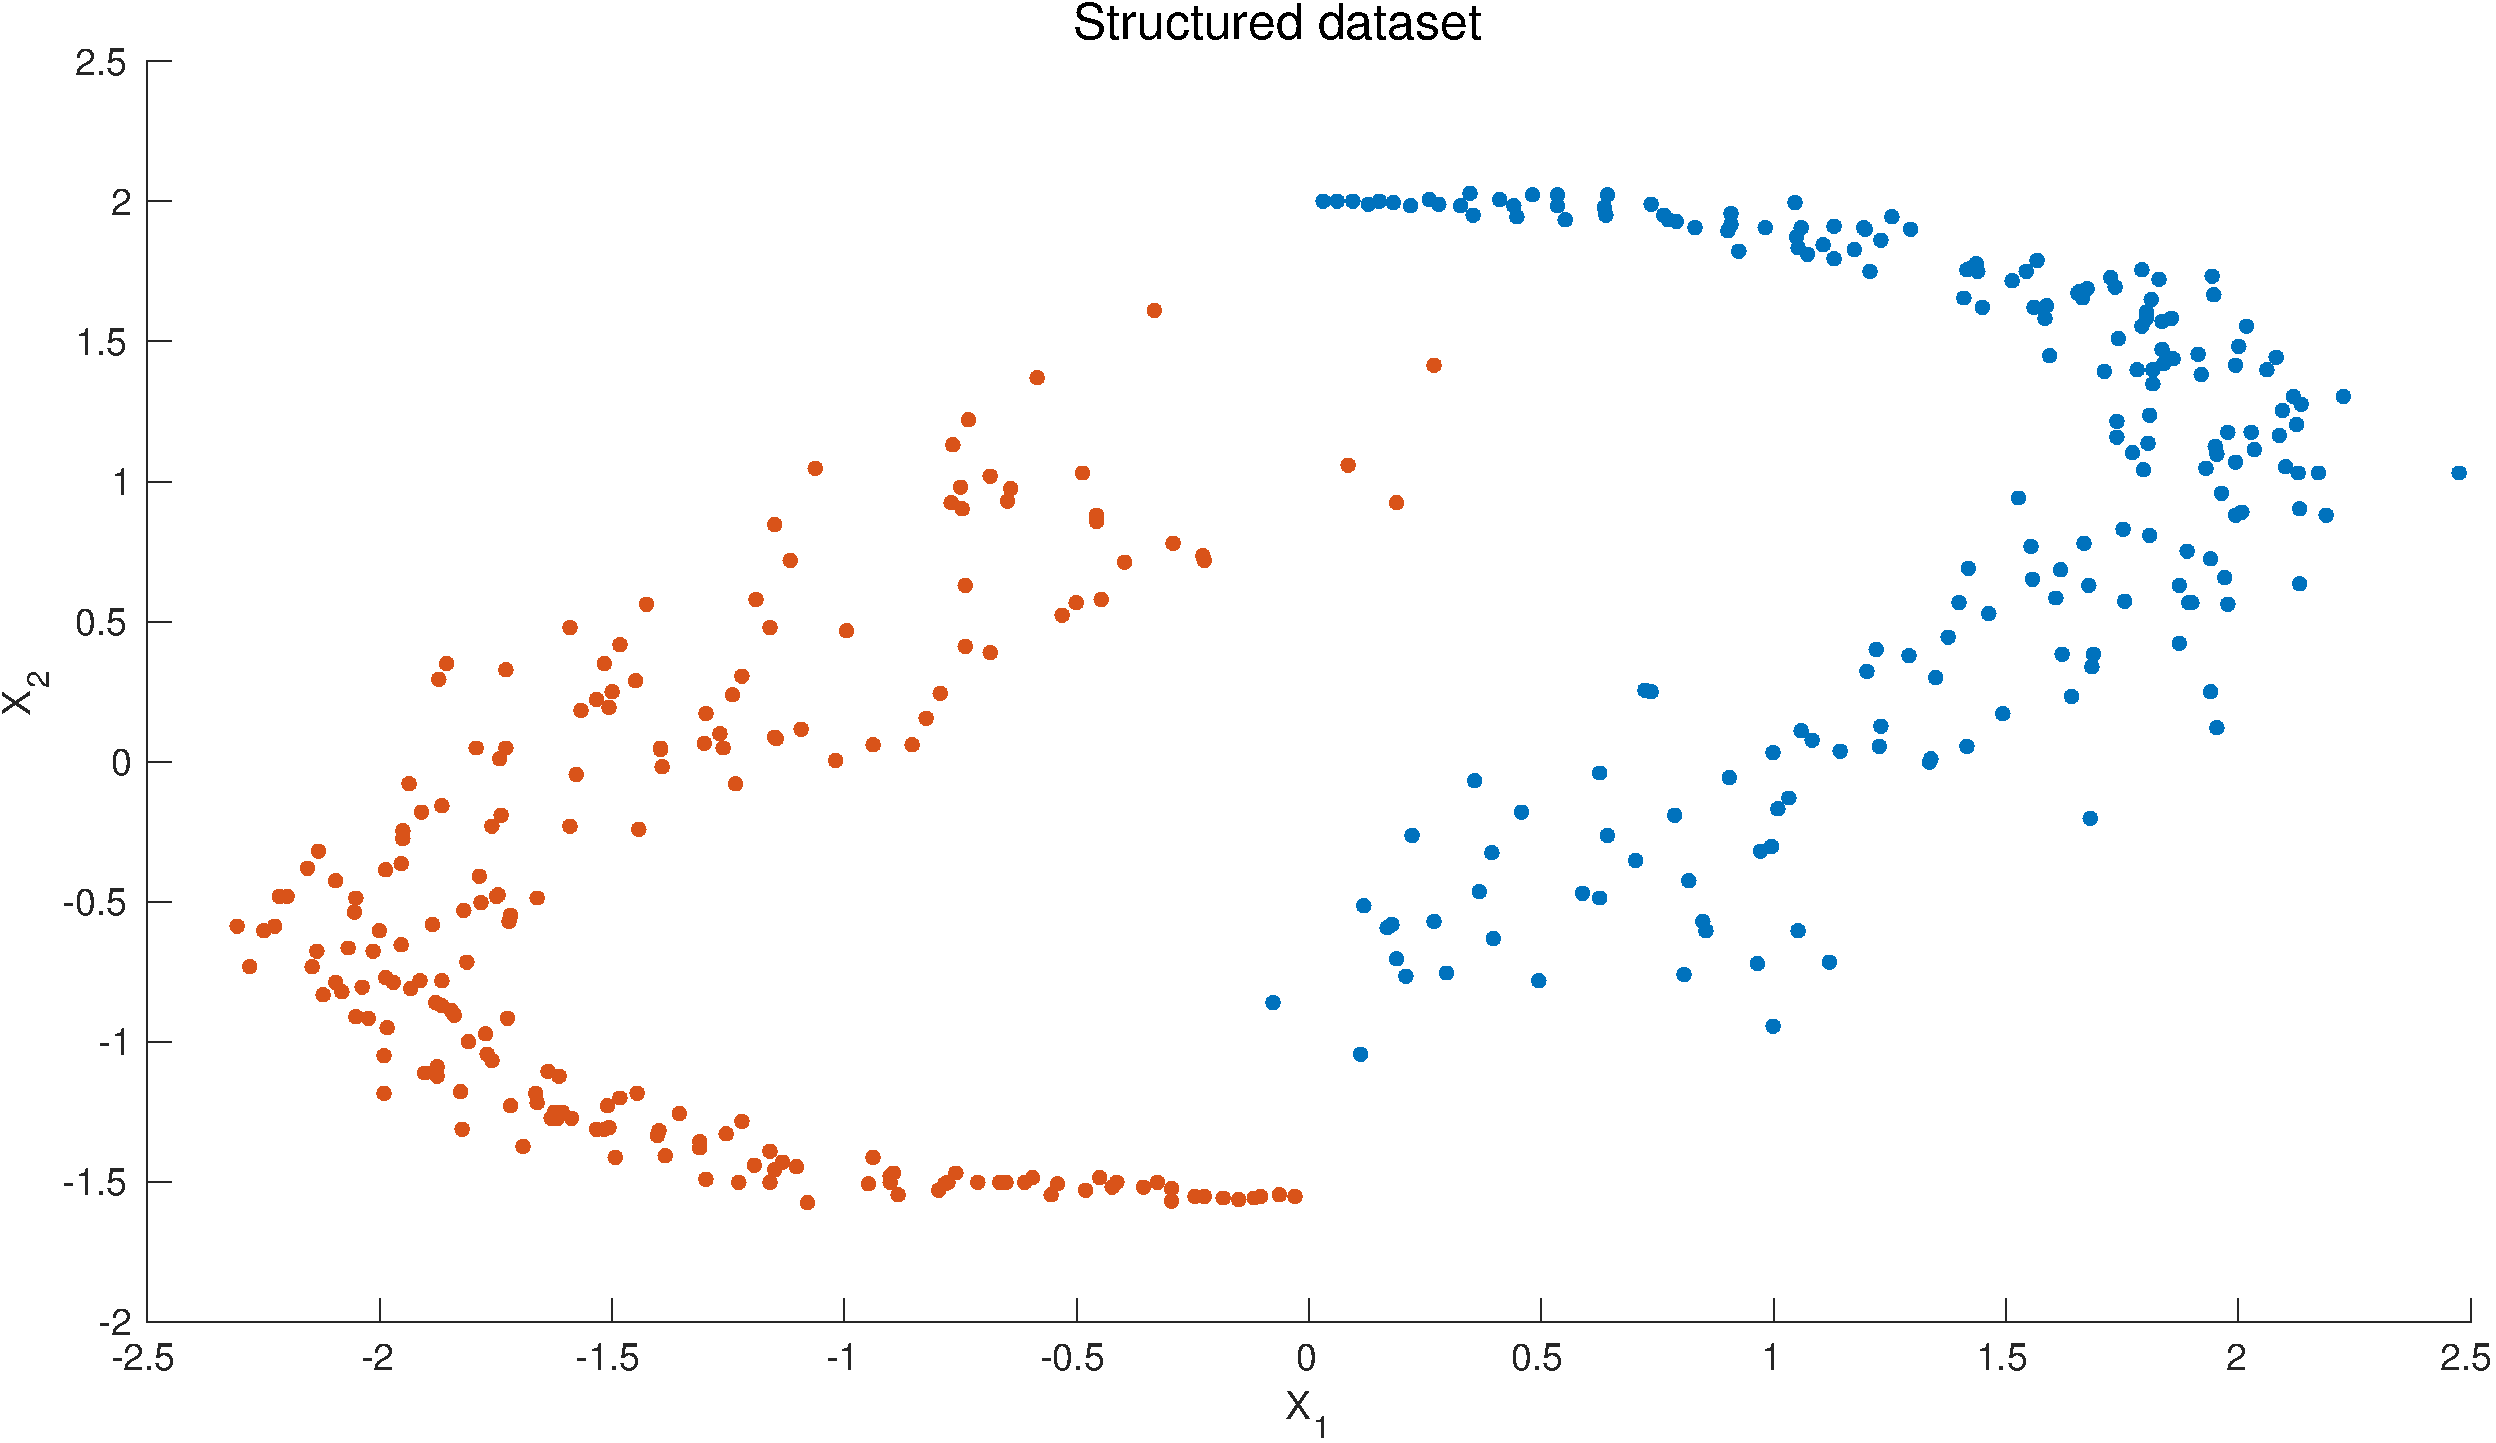
\includegraphics[scale=.40]{kpca_dataset.pdf}
  \caption{Synthetic dataset Yin-Yang}
  \label{fig:kpca_dataset}
\end{figure}

Figure \ref{fig:kpca_ncomp} allows us to visualize what happens when
you increase the number of component in a given setting (here
$\sigma^2=0.4$). We can see that the denoising works really well once
the number of components has increased to 4 and above. Figure
\ref{fig:kpca_sigma} illustrates the impact of $\sigma^2$ on the
denoising for a number of components fixed to 6. Given that the hope
is that by throwing away components, you hope to reduce the noise, a
correct choice in the number of component in this case seems to be
somewhere between 4 and 8 components. Similarly, a good value for
$\sigma^2$ seems to lie somewhere between 0.1 and 0.5.

Given the structure of the dataset, linear PCA gives very poor results
in terms of denoising (see figure \ref{fig:kpca_linear}). The maximum
amount of principal component that can be obtained using linear PCA
corresponds to the dimensionality of the original input space (p). For
the kernel PCA, the dimensionality can be higher, and is in fact
completely independent of the dimensionality of the input space. In
this setting, it corresponds to the dimensionality of the kernel
matrix (which is n-by-n, with n being the number of data point).

\begin{figure}[H]
  \centering
  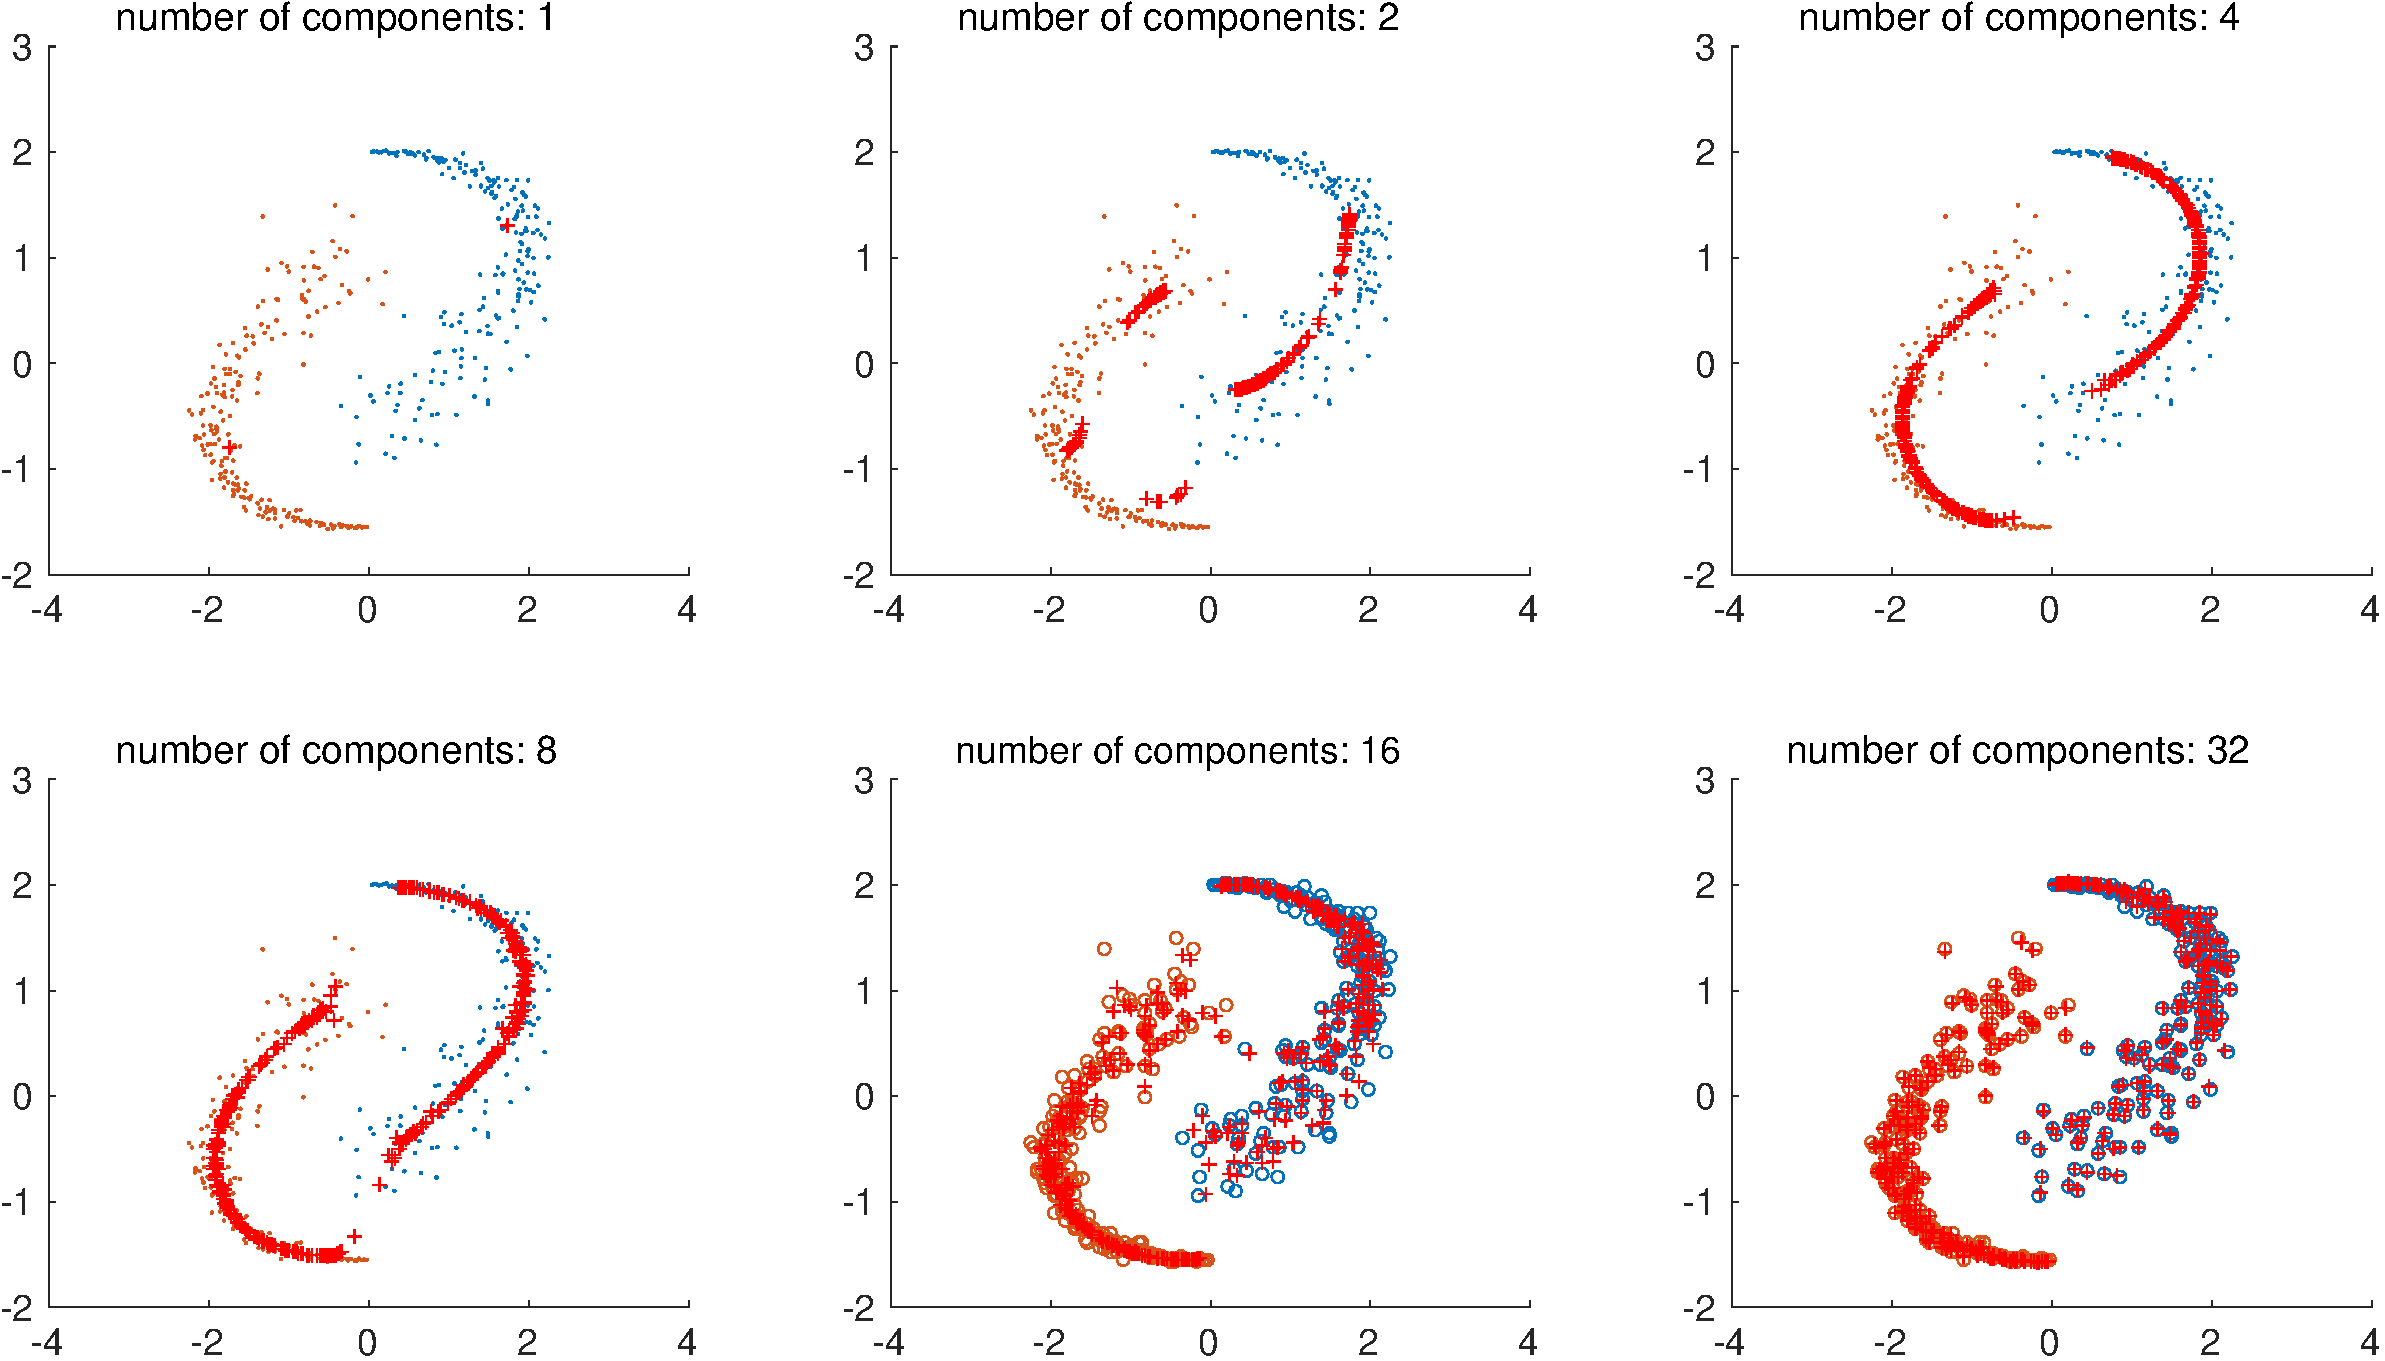
\includegraphics[scale=.40]{kpca_ncomp.pdf}
  \caption{Denoising for various values of components}
  \label{fig:kpca_ncomp}
\end{figure}

\begin{figure}[H]
  \centering
  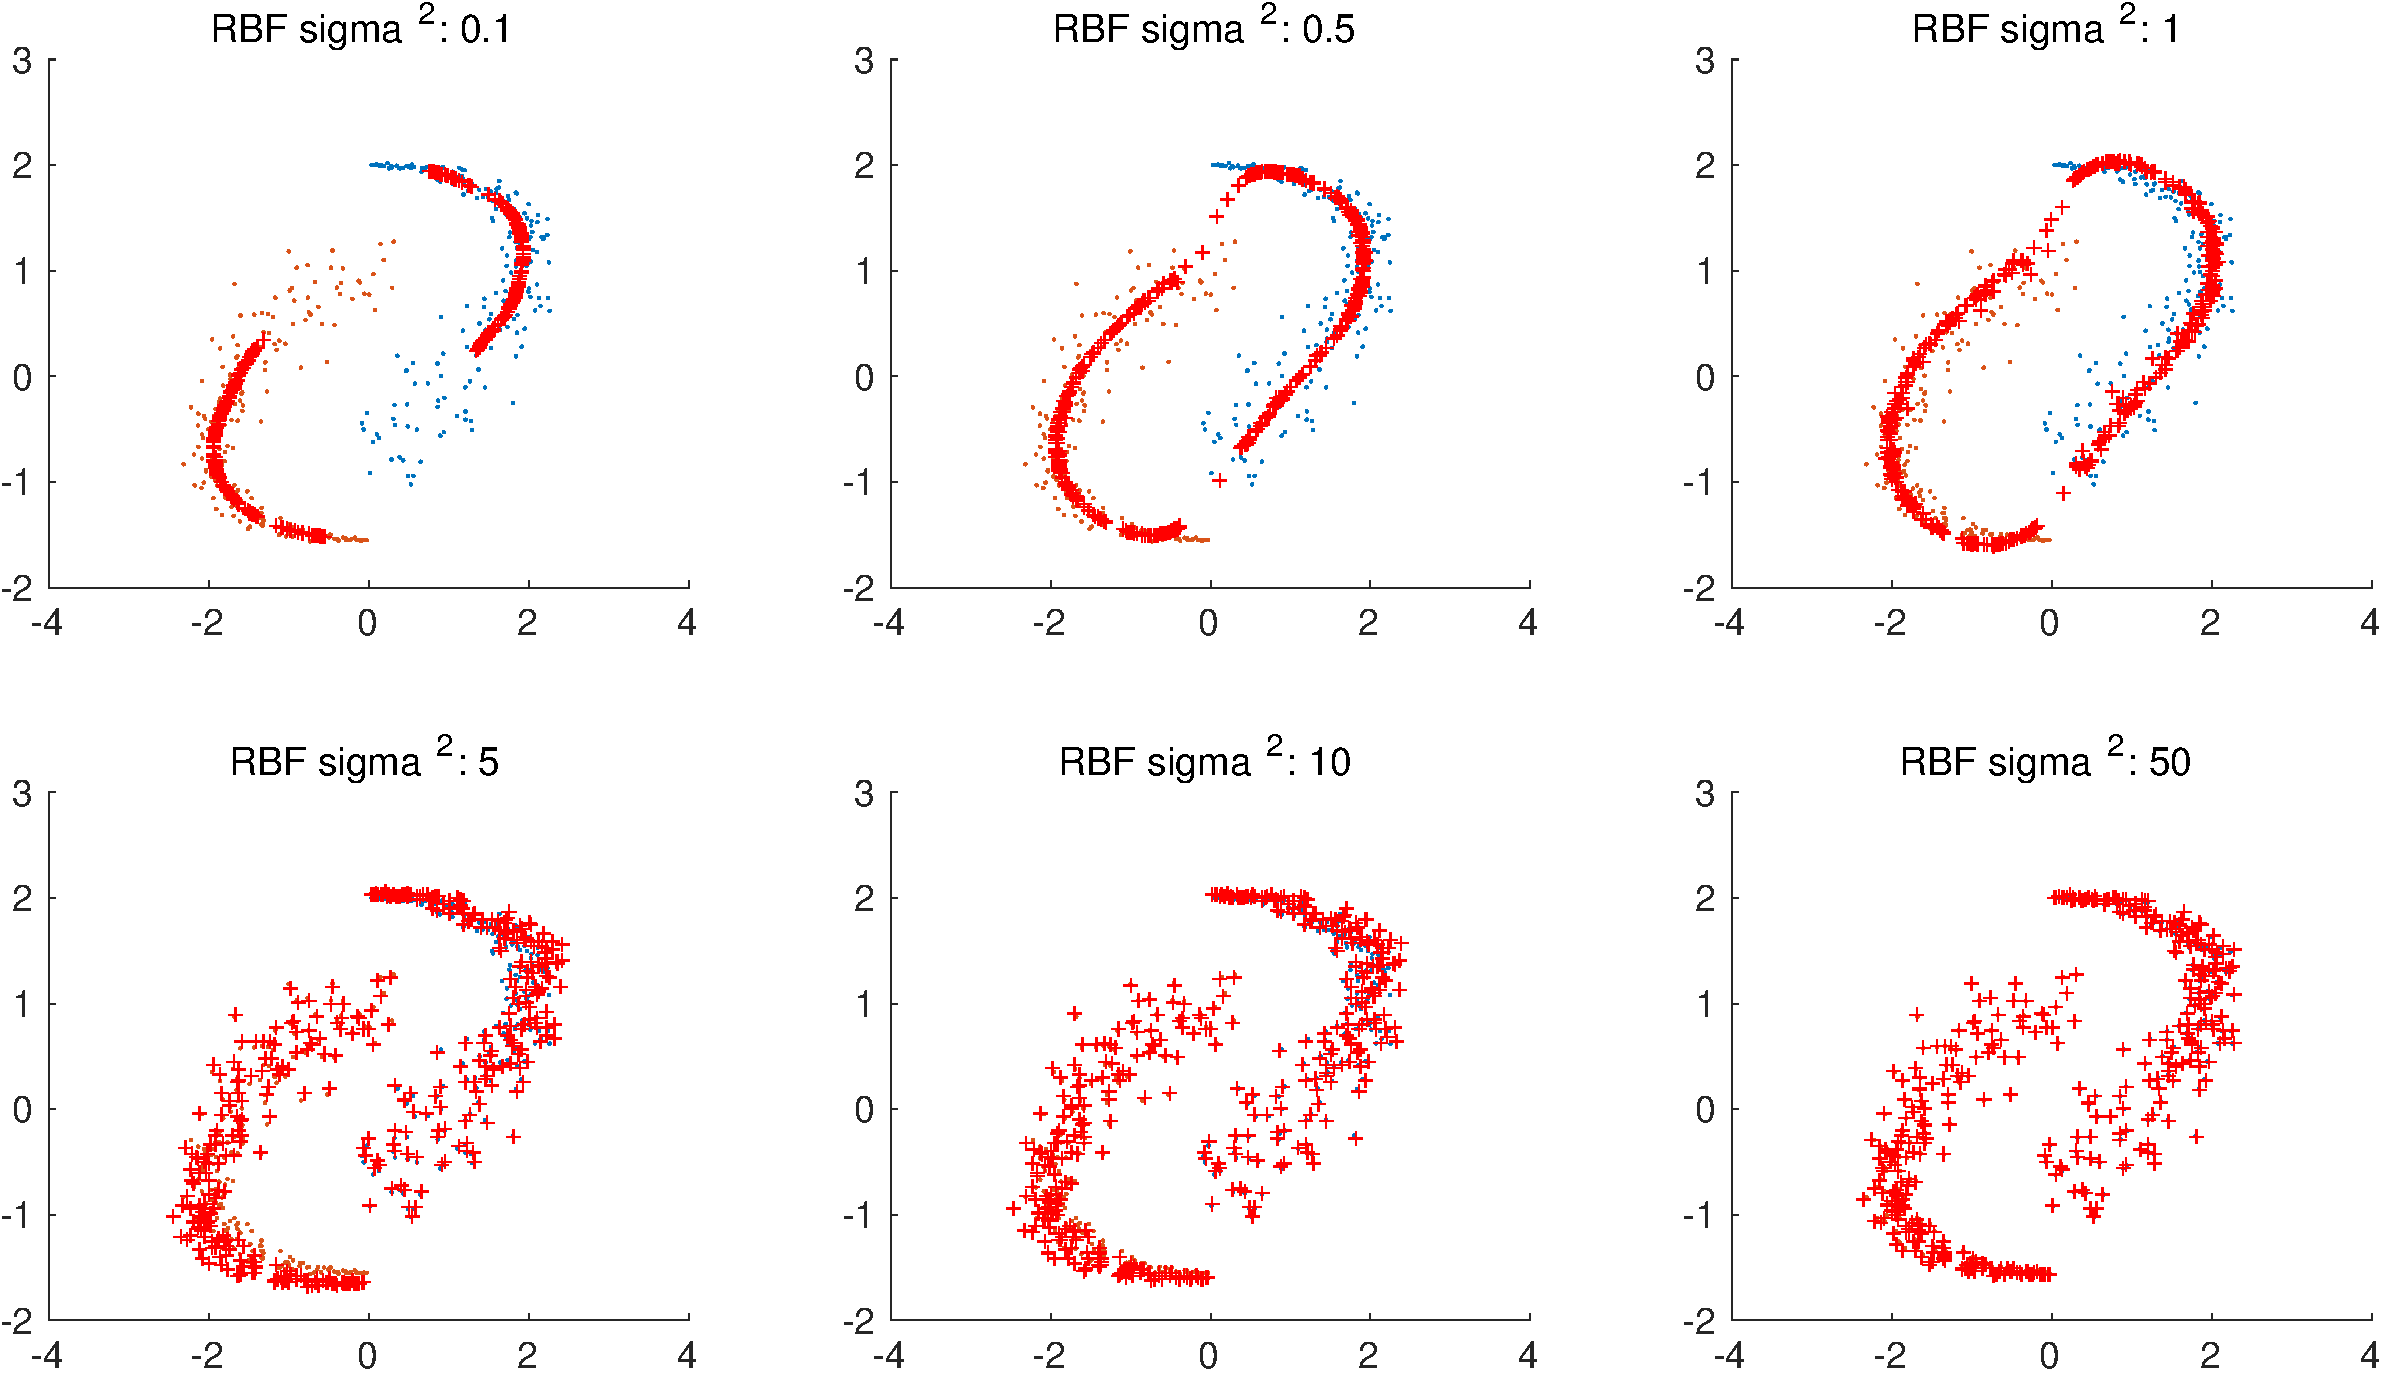
\includegraphics[scale=.40]{kpca_sigma.pdf}
  \caption{Denoising for various values of $\sigma^2$}
  \label{fig:kpca_sigma}
\end{figure}

\begin{figure}[H]
  \centering
  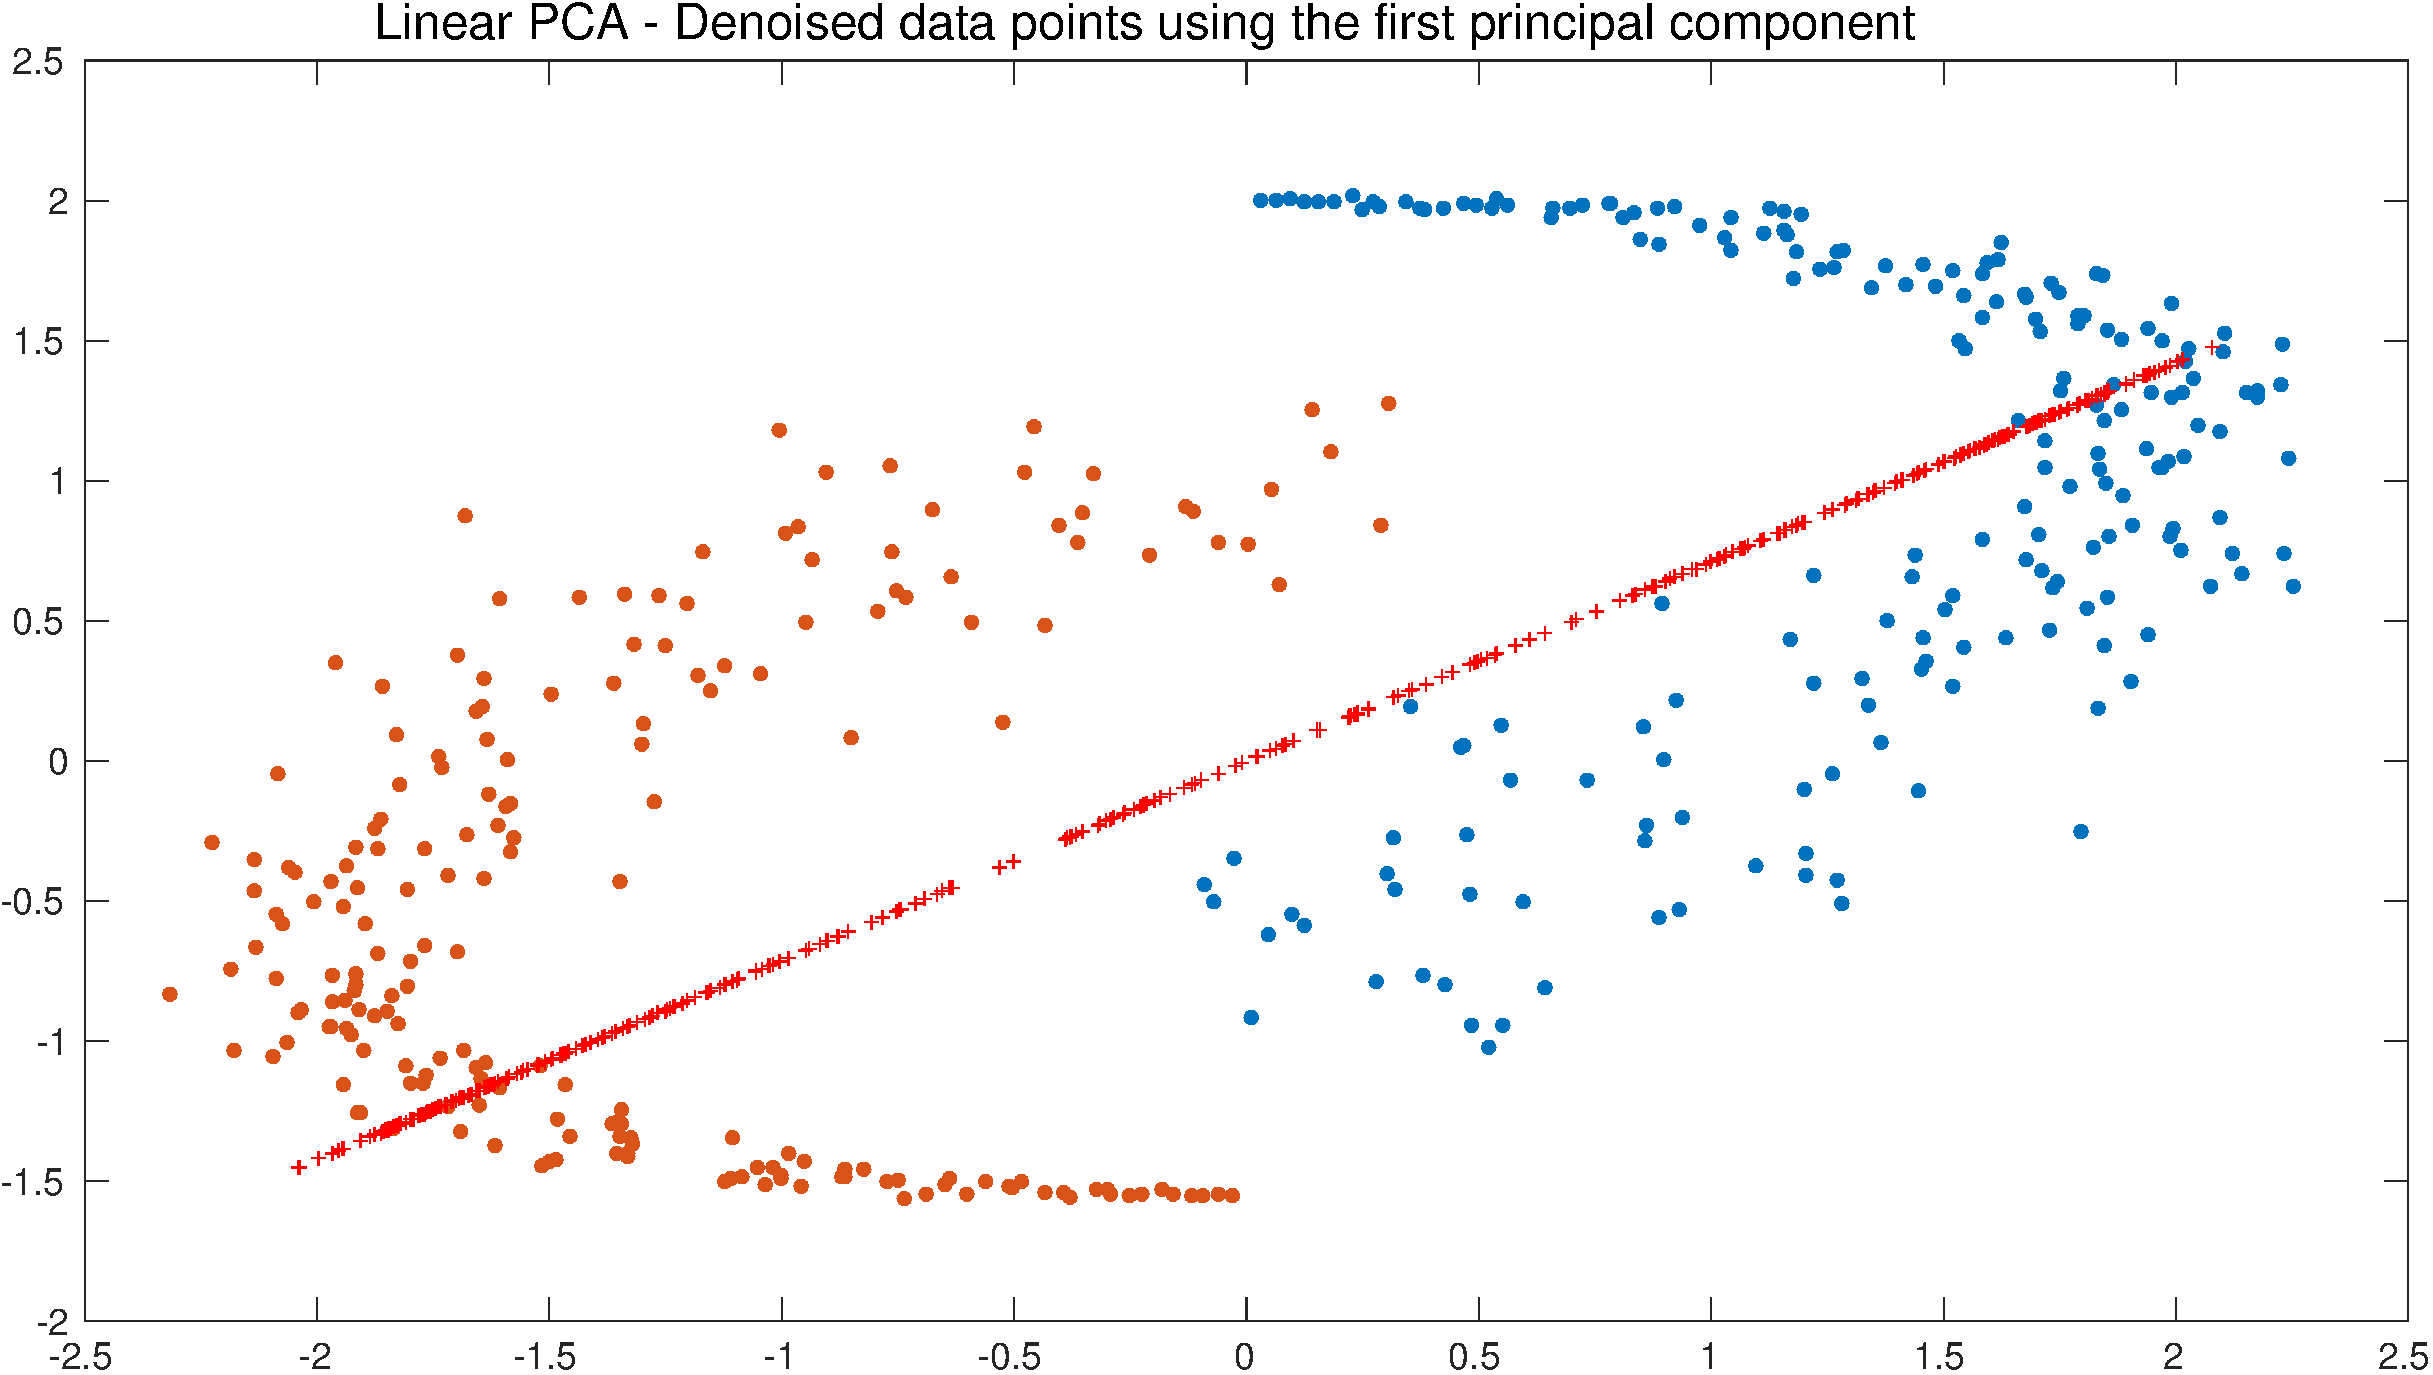
\includegraphics[scale=.30]{kpca_linear.pdf}
  \caption{Denoising in linear PCA setting}
  \label{fig:kpca_linear}
\end{figure}

A natural question is whether there is a good way to tune the number
of components and the kernel parameter, eg $\sigma^2$ in the case of a
RBF kernel. I would say that one way to proceed would be to
systematically compute the error between a denoised model trained on a
part of the dataset (training set), then compute the error made using
the test set. In the example above, it is easy to see that with very
high number of components or a large $\sigma^2$ would result in a
fitting of the noise. Given that we know the underlying true function,
a calculation of the error would reveal the overfitting.

\section{Handwritten Digit Denoising}

The results of the denoising process are reported on figures
\ref{fig:digitsn_kernelpca} and \ref{fig:digitsn_linearpca}. As can be
observed, the performance of the kernel PCA in terms of denoising are
much better. Basically, the linear PCA decomposition into 256
components, followed by the reconstruction using progressively more
and more components (256 in the last row) returns the original noisy
image. Where as the kernel PCA is able to extract out the gaussian
noise during the reconstruction, returning a very convincing, denoised
image which is similar to the original noiseless one.

Interestingly, it is possible to see some errors in the reconstruction
of the digits using the kernel PCA approach, indicating that a certain
amount of components is necessary. For many of the digits it would
seem that using very few components for the reconstruction leads to a
8 and a 7. Increasing the components resolves the problem for most
digits.

\begin{figure}[H]
  \centering
  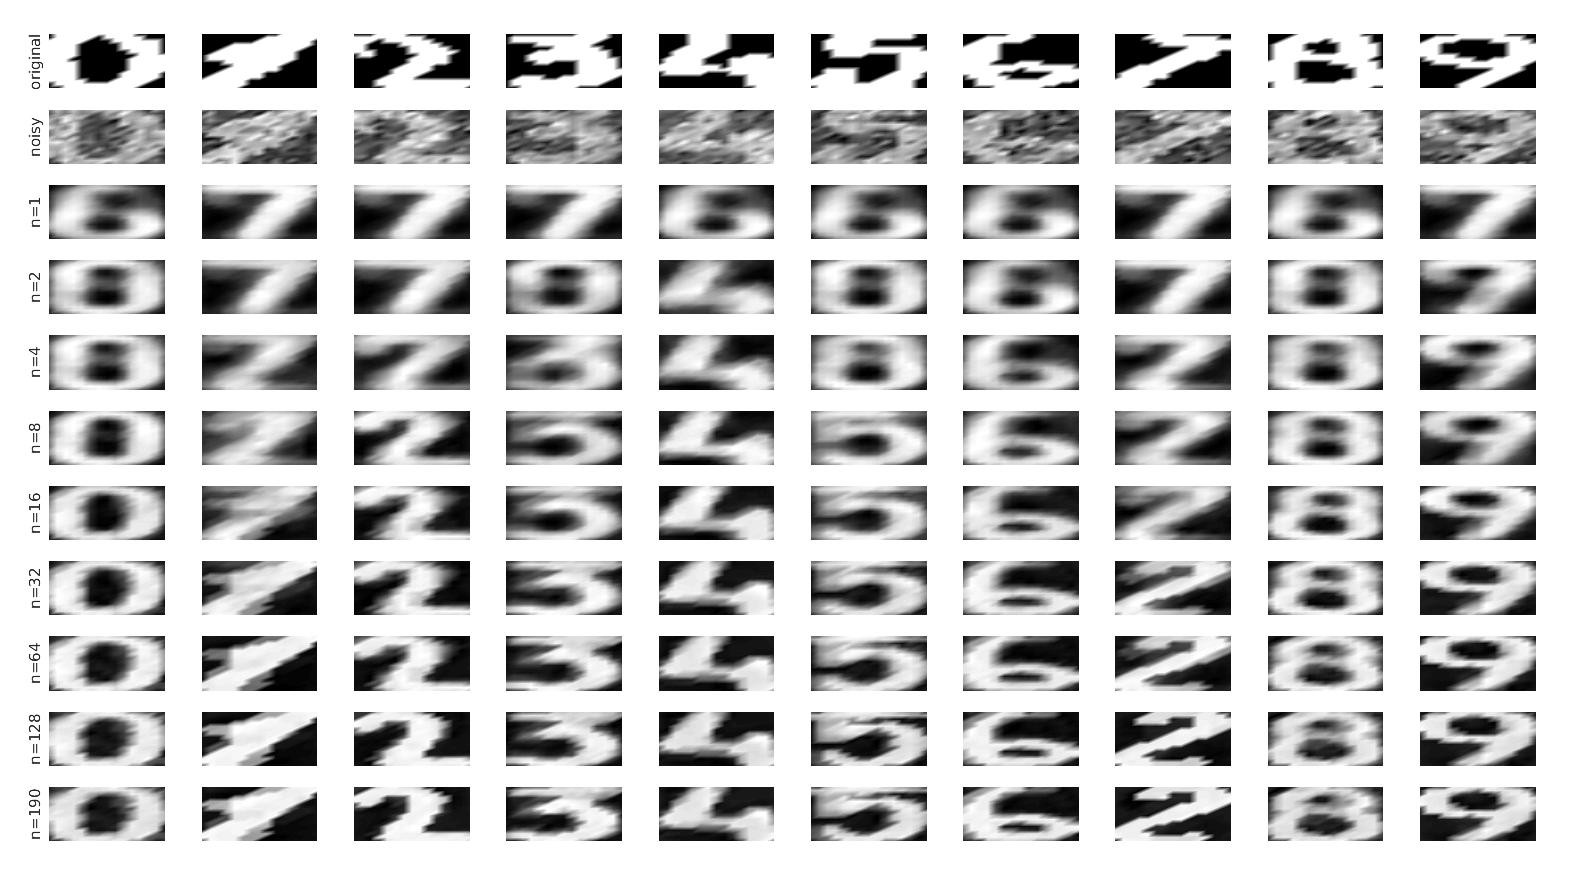
\includegraphics[scale=.30]{digitsn_kernelpca.jpg}
  \caption{Denoising digits using a kernel PCA approach}
  \label{fig:digitsn_kernelpca}
\end{figure}

\begin{figure}[H]
  \centering
  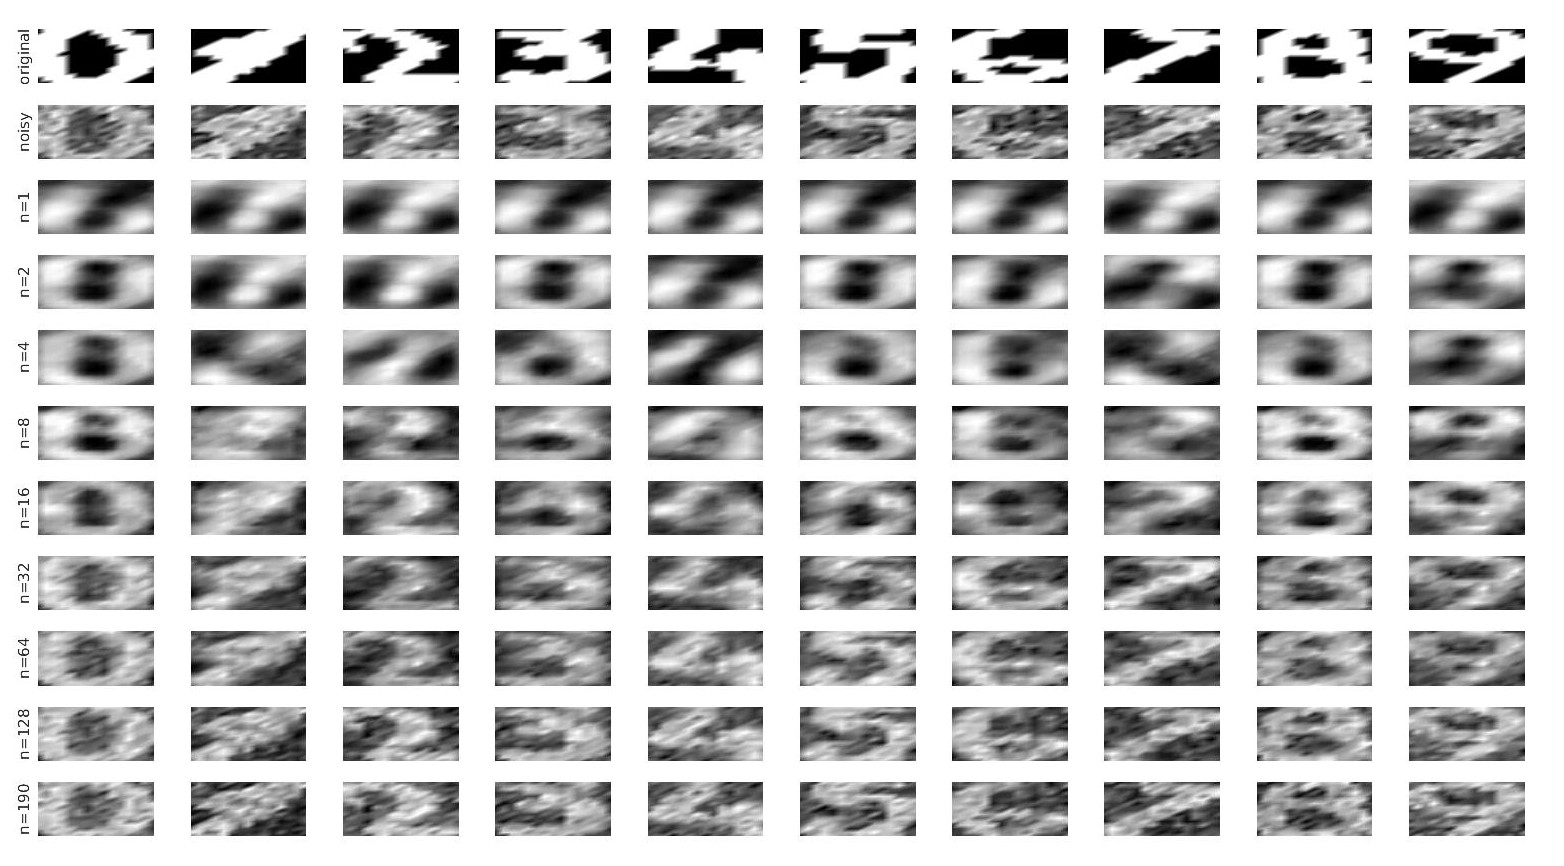
\includegraphics[scale=.30]{digitsn_linearpca.jpg}
  \caption{Denoising digits using a linear PCA approach}
  \label{fig:digitsn_linearpca}
\end{figure}

\section{Spectral Clustering}

The difference between clustering and classification lies in the type
of learning at work. In clustering, no labels are used - a setting
usually referred to as \emph{unsupervised learning}.

On the figure \ref{fig:sclustering_origcl} and
\ref{fig:sclustering_matrix} we can see the results fo the spectral
clustering for various values of $\sigma^2$. A good value $\sigma^2$
seem to lead to good clustering results, ie a good separation of the
two rings.

\begin{figure}[H]
  \centering
  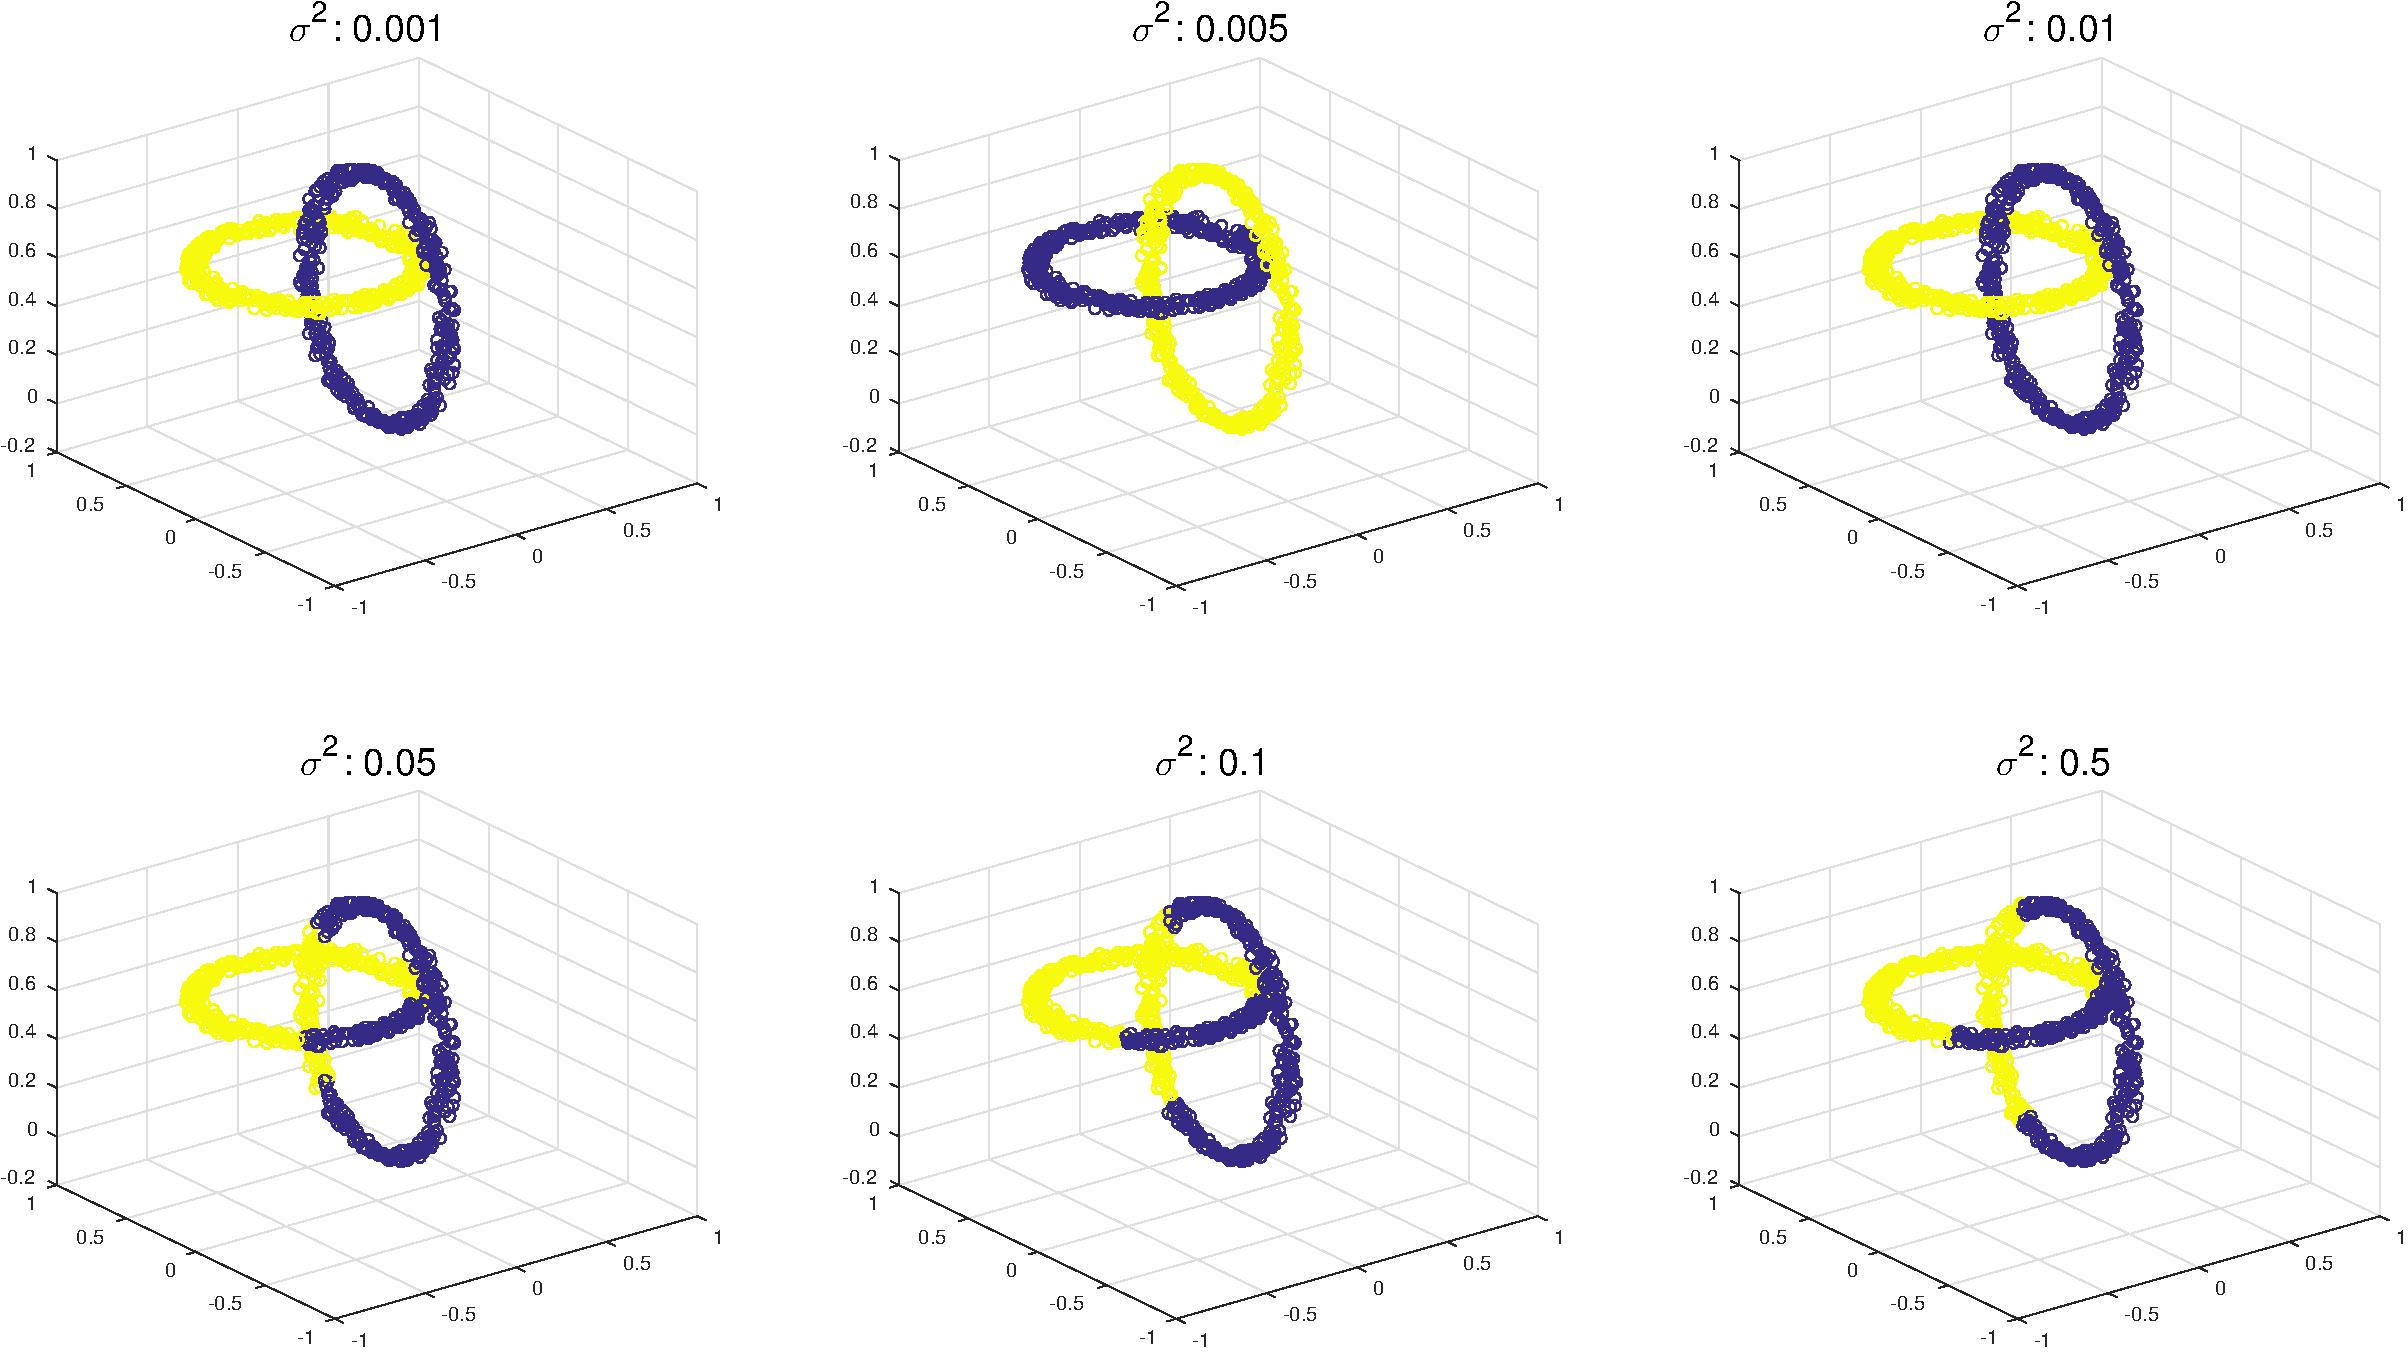
\includegraphics[scale=.40]{sclustering_origcl.pdf}
  \caption{Clustering 1}
  \label{fig:sclustering_origcl}
\end{figure}

\begin{figure}[H]
  \centering
  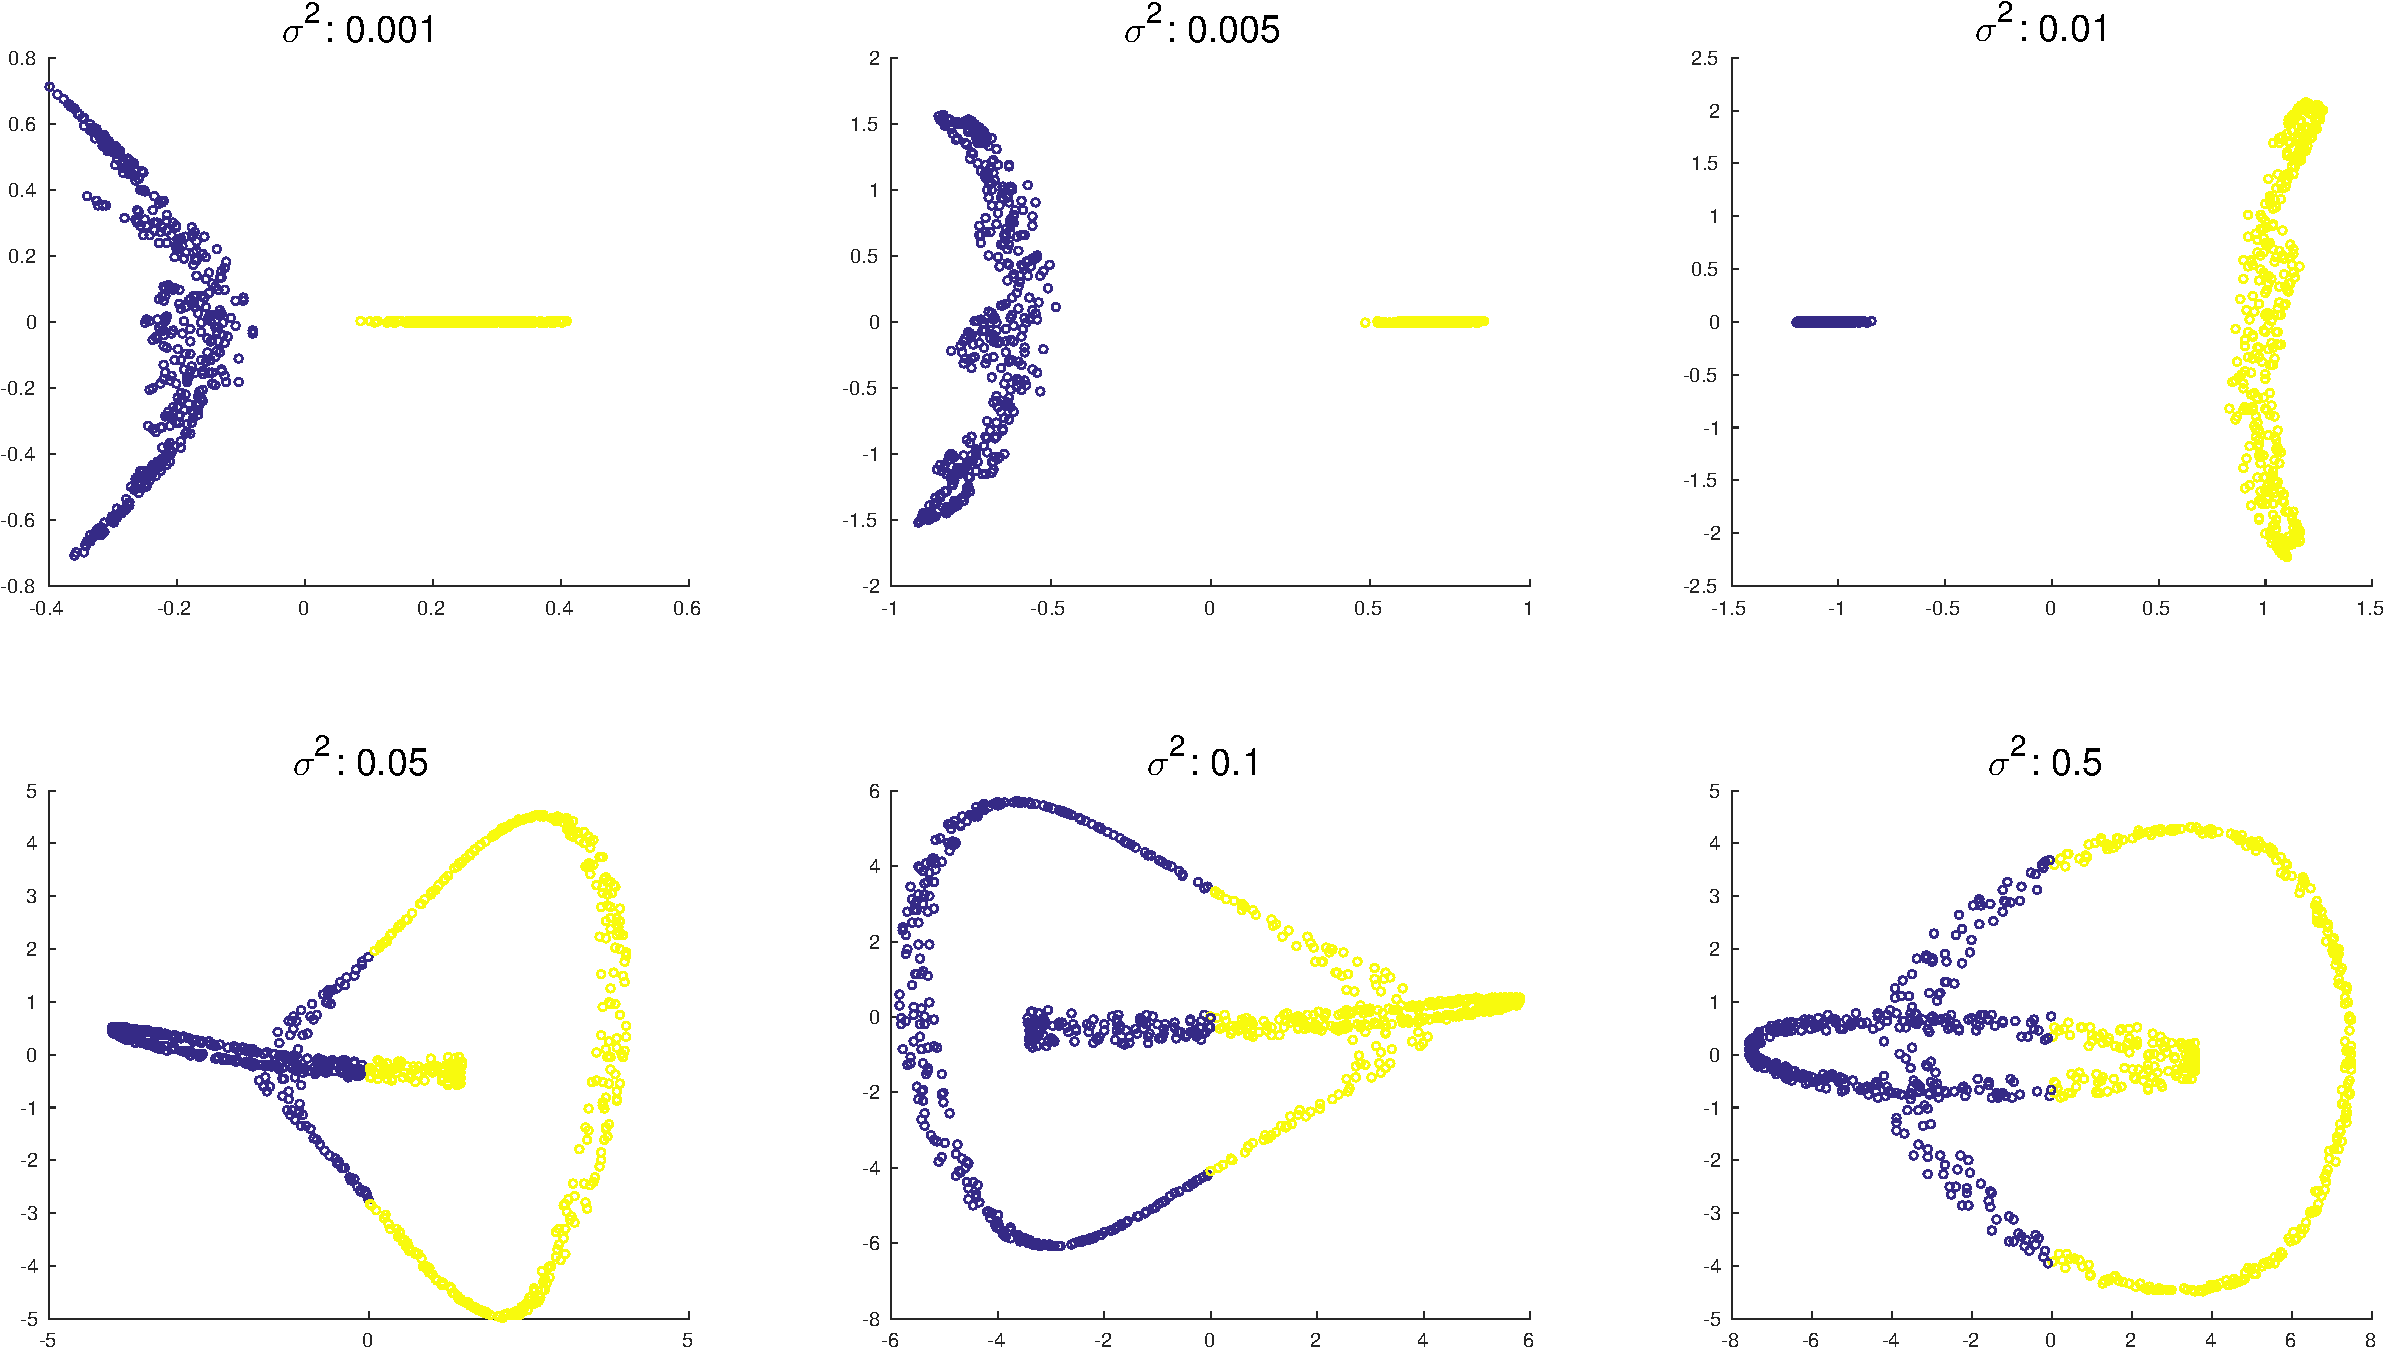
\includegraphics[scale=.40]{sclustering_origcl2.pdf}
  \caption{Clustering 2}
  \label{fig:sclustering_origcl2}
\end{figure}

Figure \ref{fig:sclustering_matrix} reports the kernel matrix for a
value of $\sigma^2=0.05$, this is a bit suboptimal, but the better
value $\sigma^2=0.005$ gave a rendering that is mostly dark (lots of
support vector, matrix not sparse) which did not render well. 


\begin{figure}[H]
  \centering
  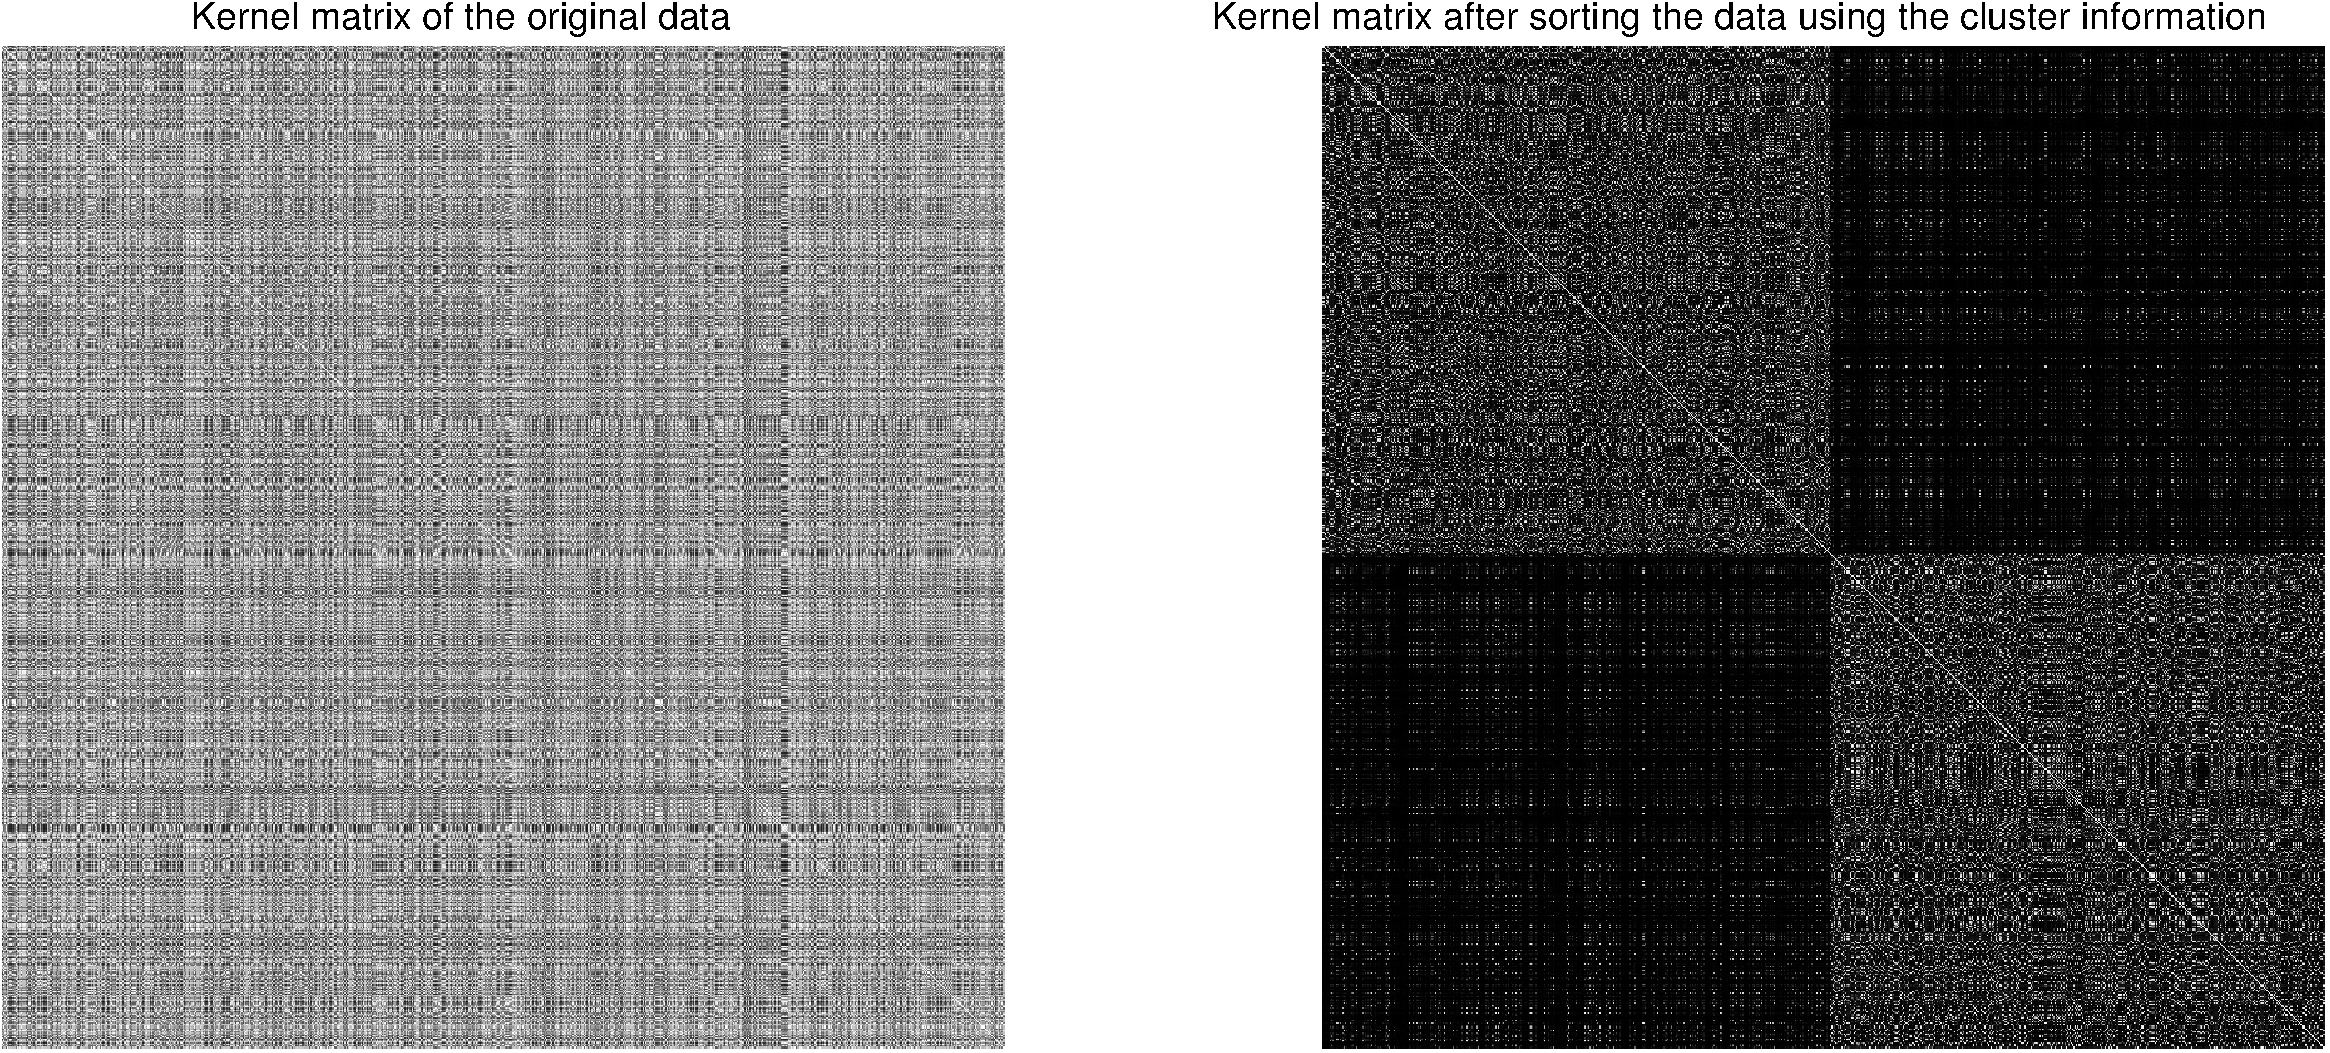
\includegraphics[scale=.40]{scluster_matrix.pdf}
  \caption{Matrix}
  \label{fig:sclustering_matrix}
\end{figure}

\section{Fixed-size LS-SVM}

In this section, we use a Nystrom approximation of the feature
map. This allows us to construct parametric models in the primal
space. By means of finite samples of the datapoints, one can obtain a
finite estimation of the feature map.

Figure \ref{fig:fslssvm_sig2} reports the influence of different
values of $\sigma^2$ on the subset selection. Larger values of
$\sigma^2$ seem to result in a selection that is more evenly spaced.

\begin{figure}[H]
  \centering
  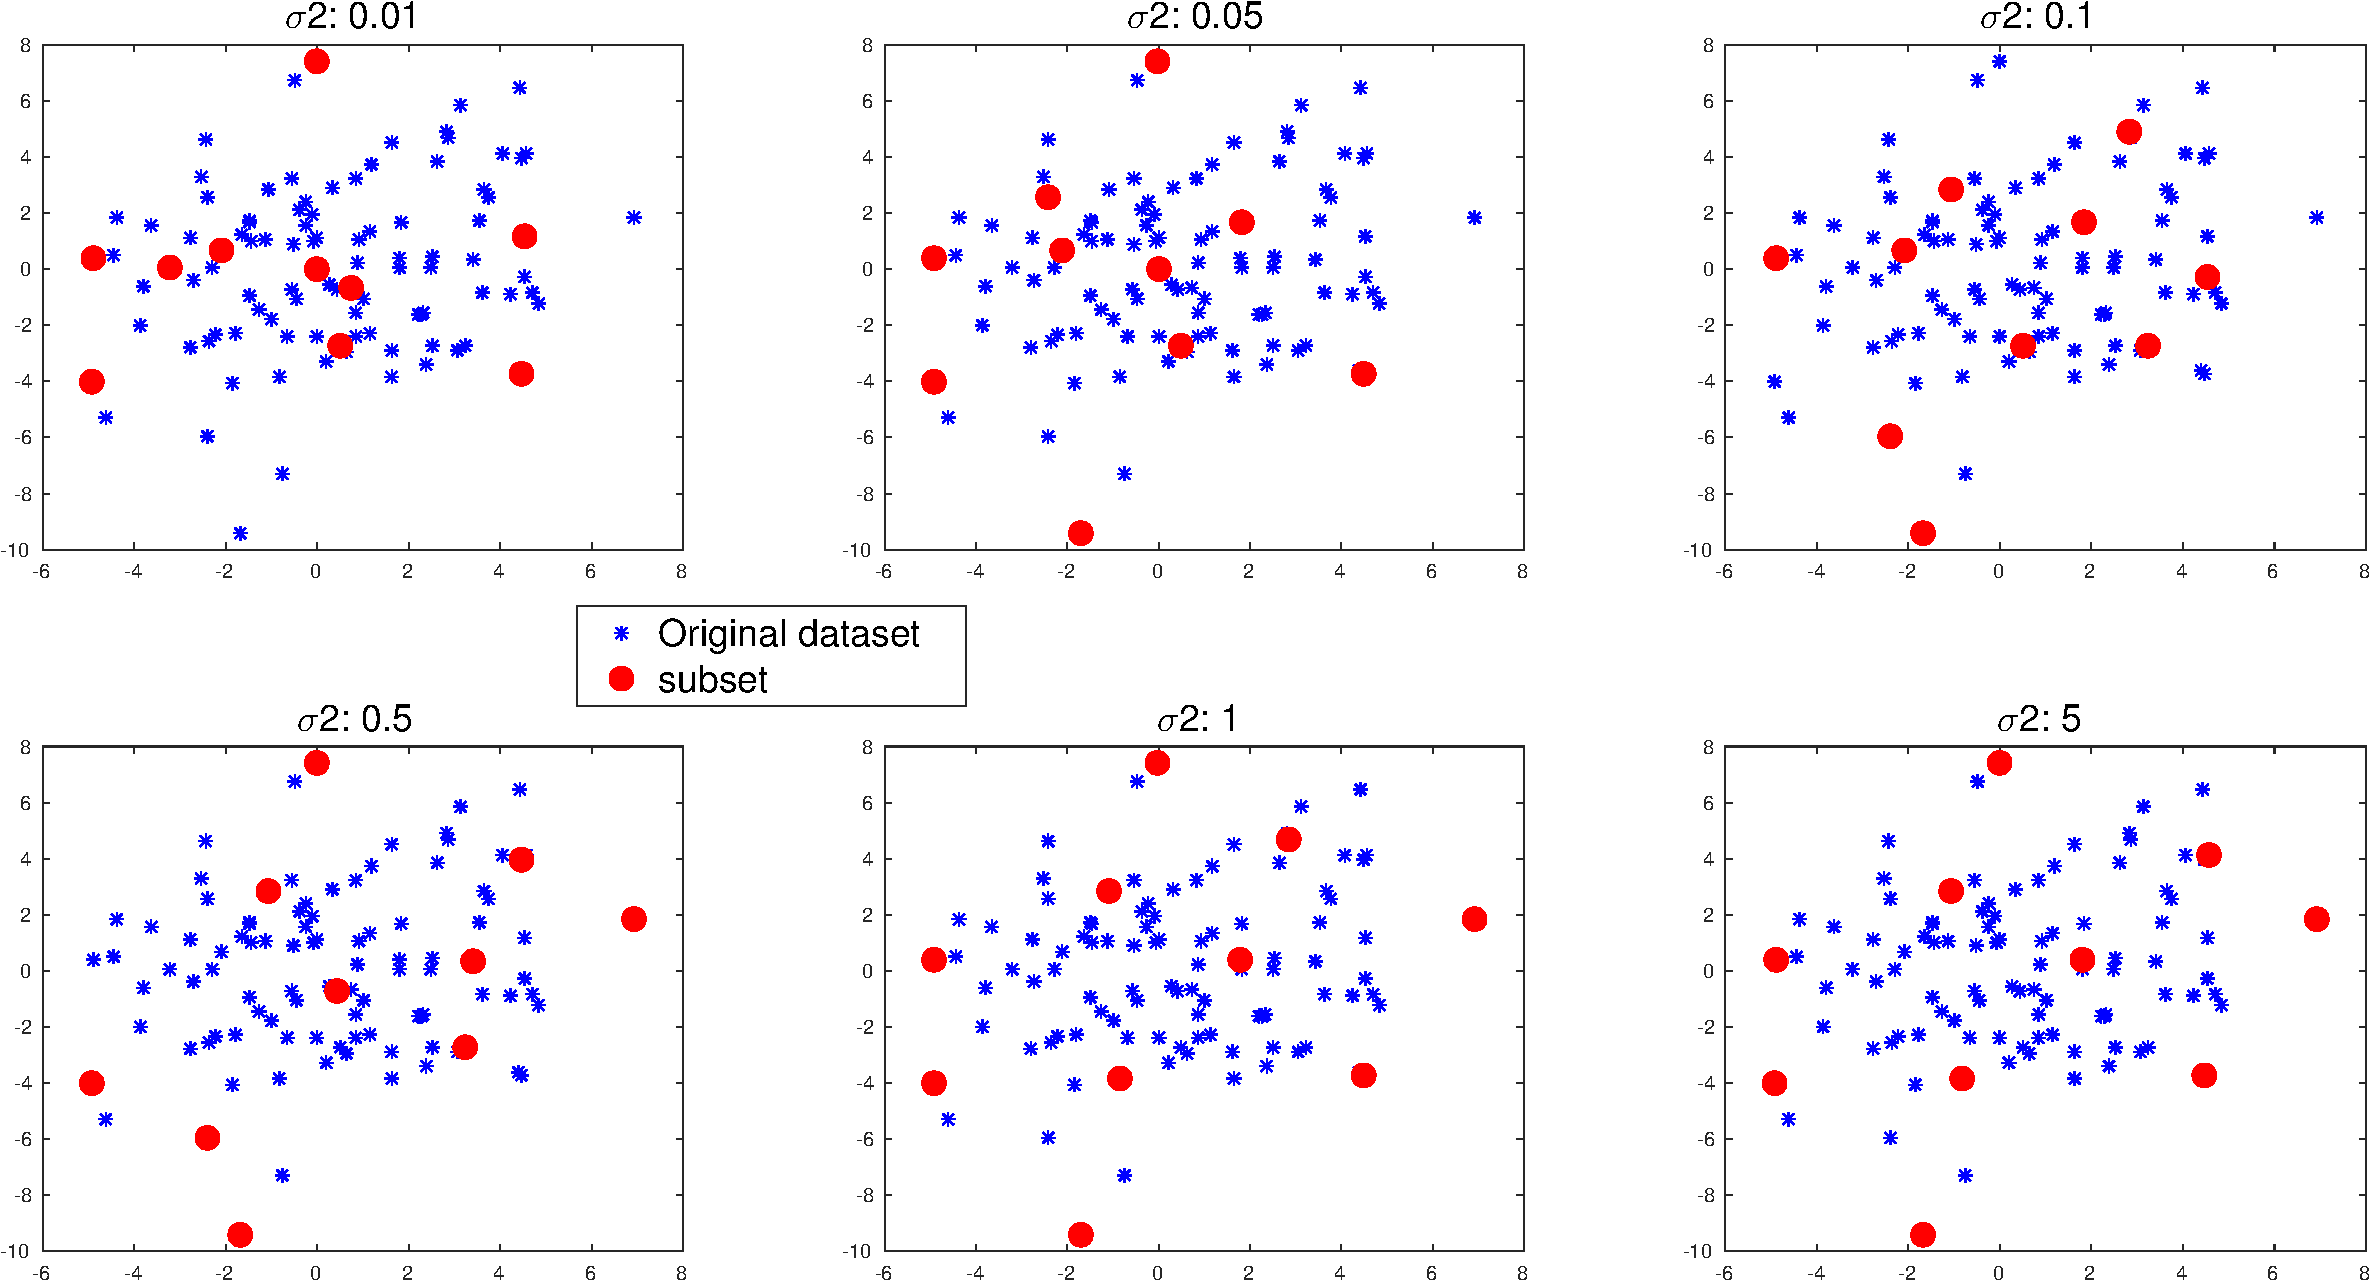
\includegraphics[scale=.40]{fslssvm_sig2.pdf}
  \caption{Subset selection via fixed-size lssvm}
  \label{fig:fslssvm_sig2}
\end{figure}

Figure \ref{fig:fslssvm_script} shows the results in terms of
different metrics for the two approaches, fixed-size lssvm and the
$l_0-approximation$.

\begin{figure}[H]
  \centering
  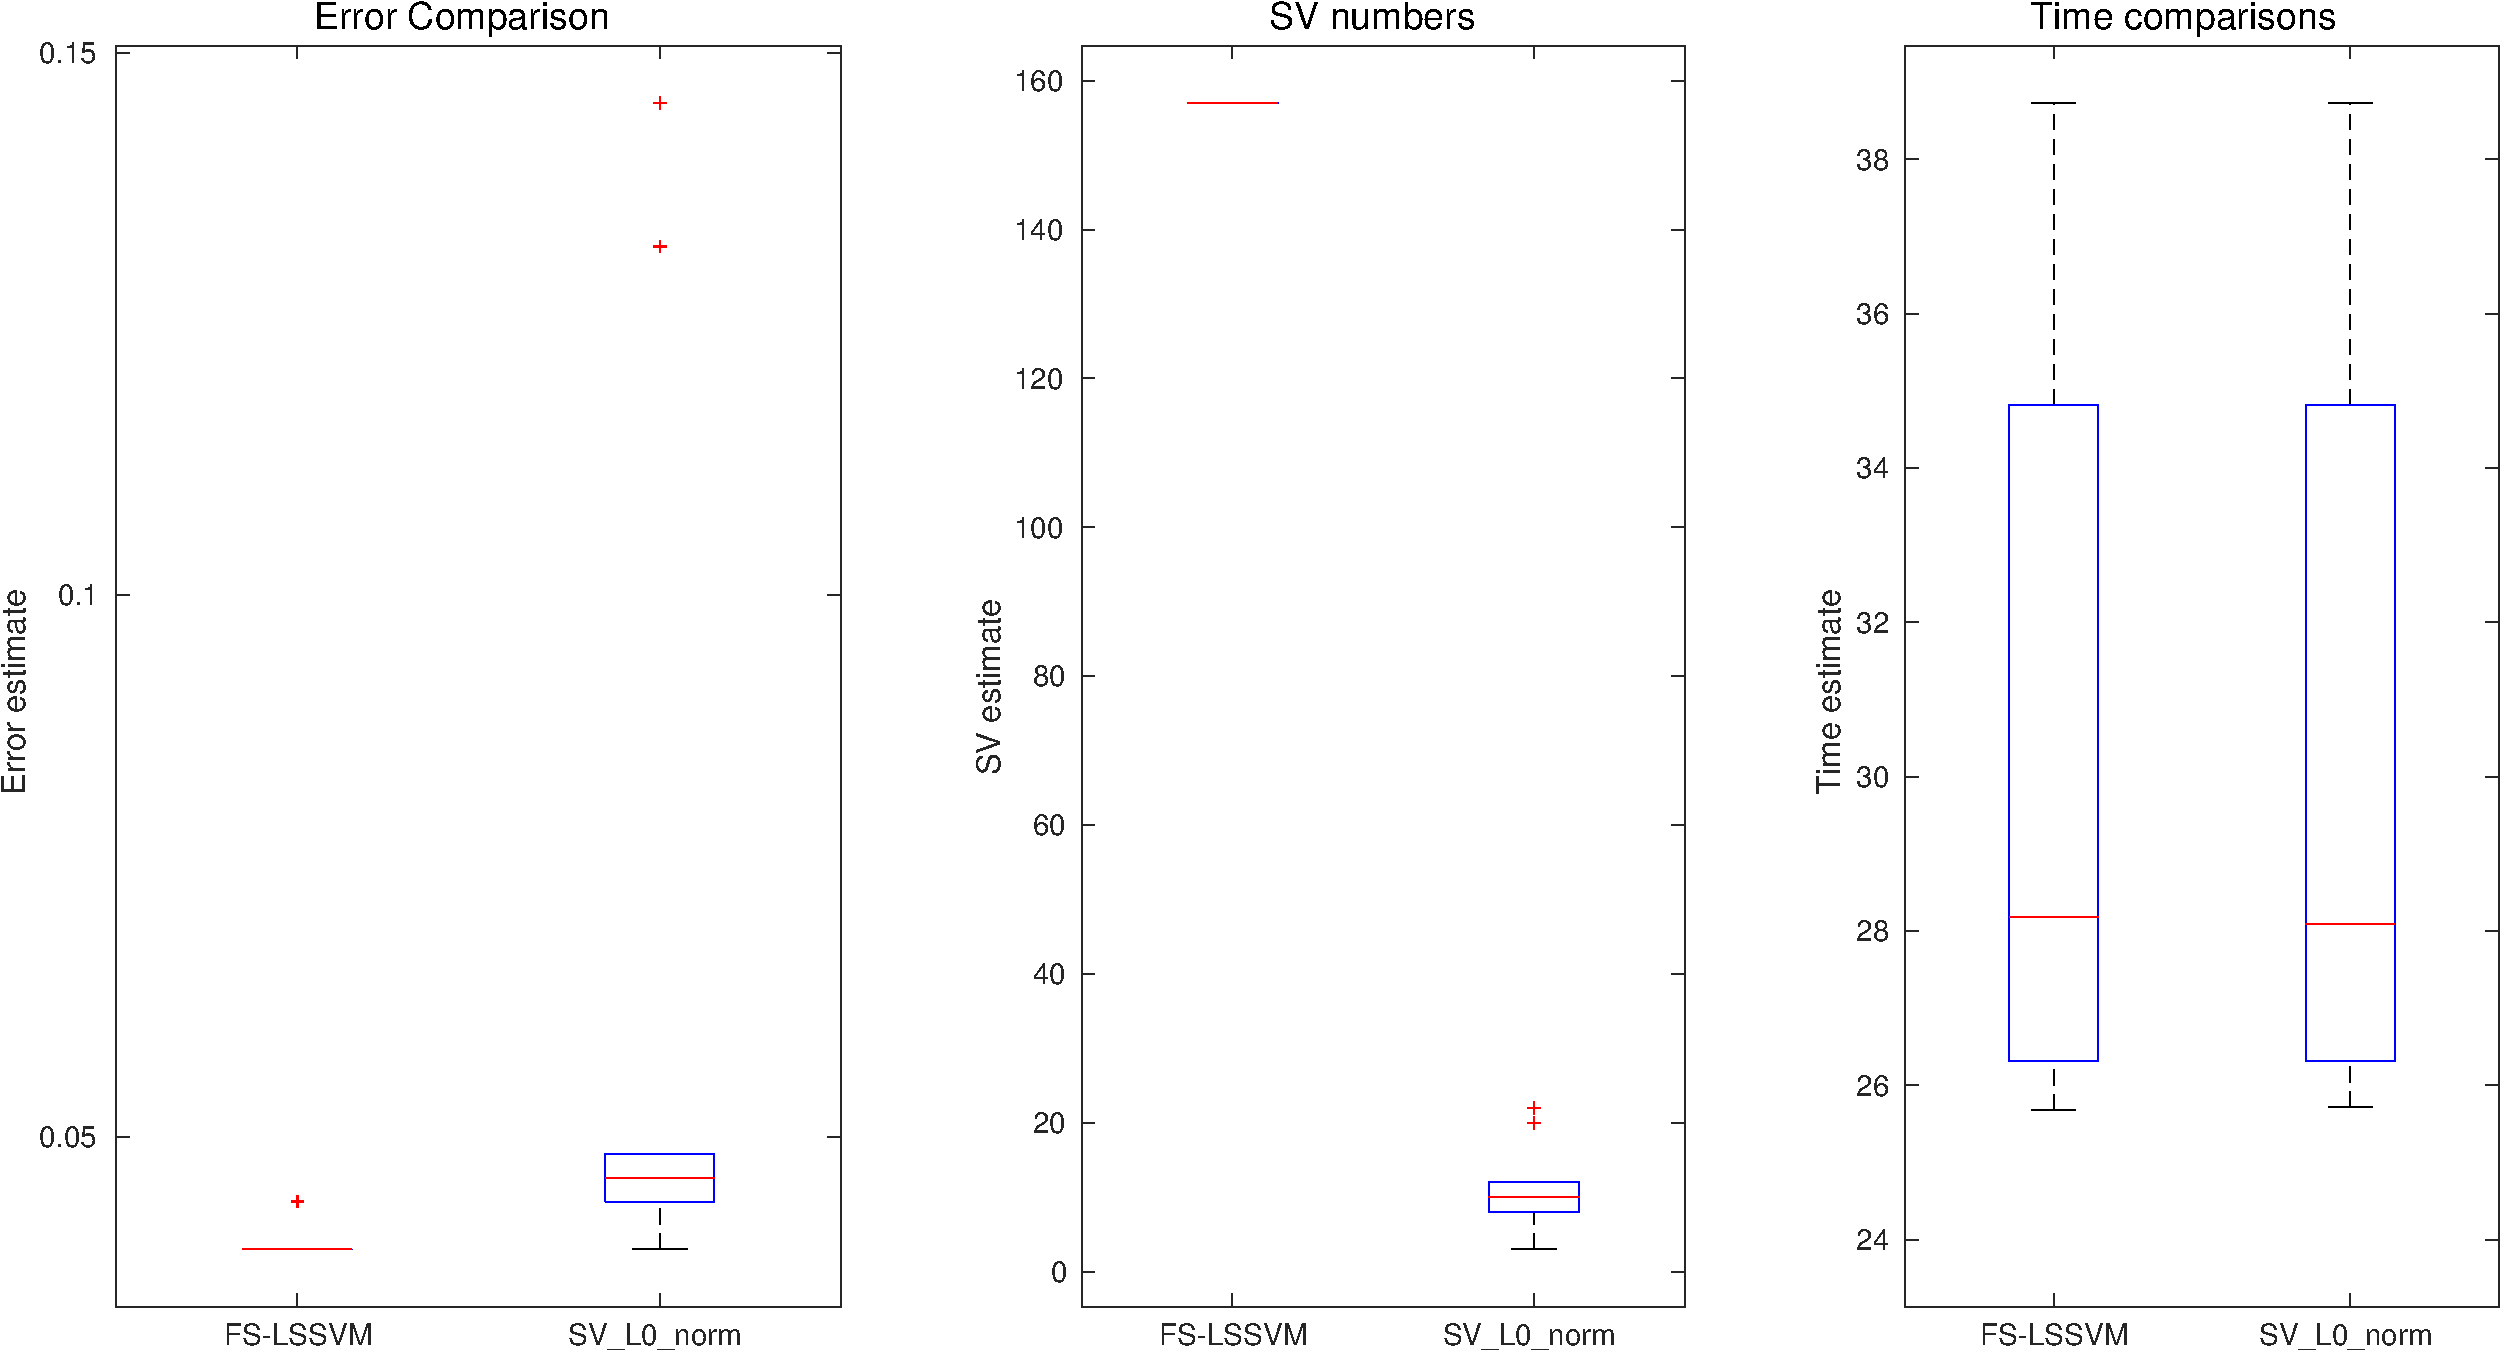
\includegraphics[scale=.40]{fslssvm_script.pdf}
  \caption{fslssvm-script}
  \label{fig:fslssvm_script}
\end{figure}


\section{Applications}

\subsection{Handwritten Digit Denoising}

Here we revisit the denoising of the handwritten digit. First, I
explored the impact of the value of the $\sigma^2$ parameter on the
denoising. The results are reported on the figure
\ref{fig:nndigits_all} below. As you can see, with larger values of
$\sigma^2$, the reconstruction process through which the noise is
eliminated tends to decrease in efficiency. For exagerately large
values of the parameter, the reconstruction is not legible, and
consists only of noise.

\begin{figure}[H]
  \centering
  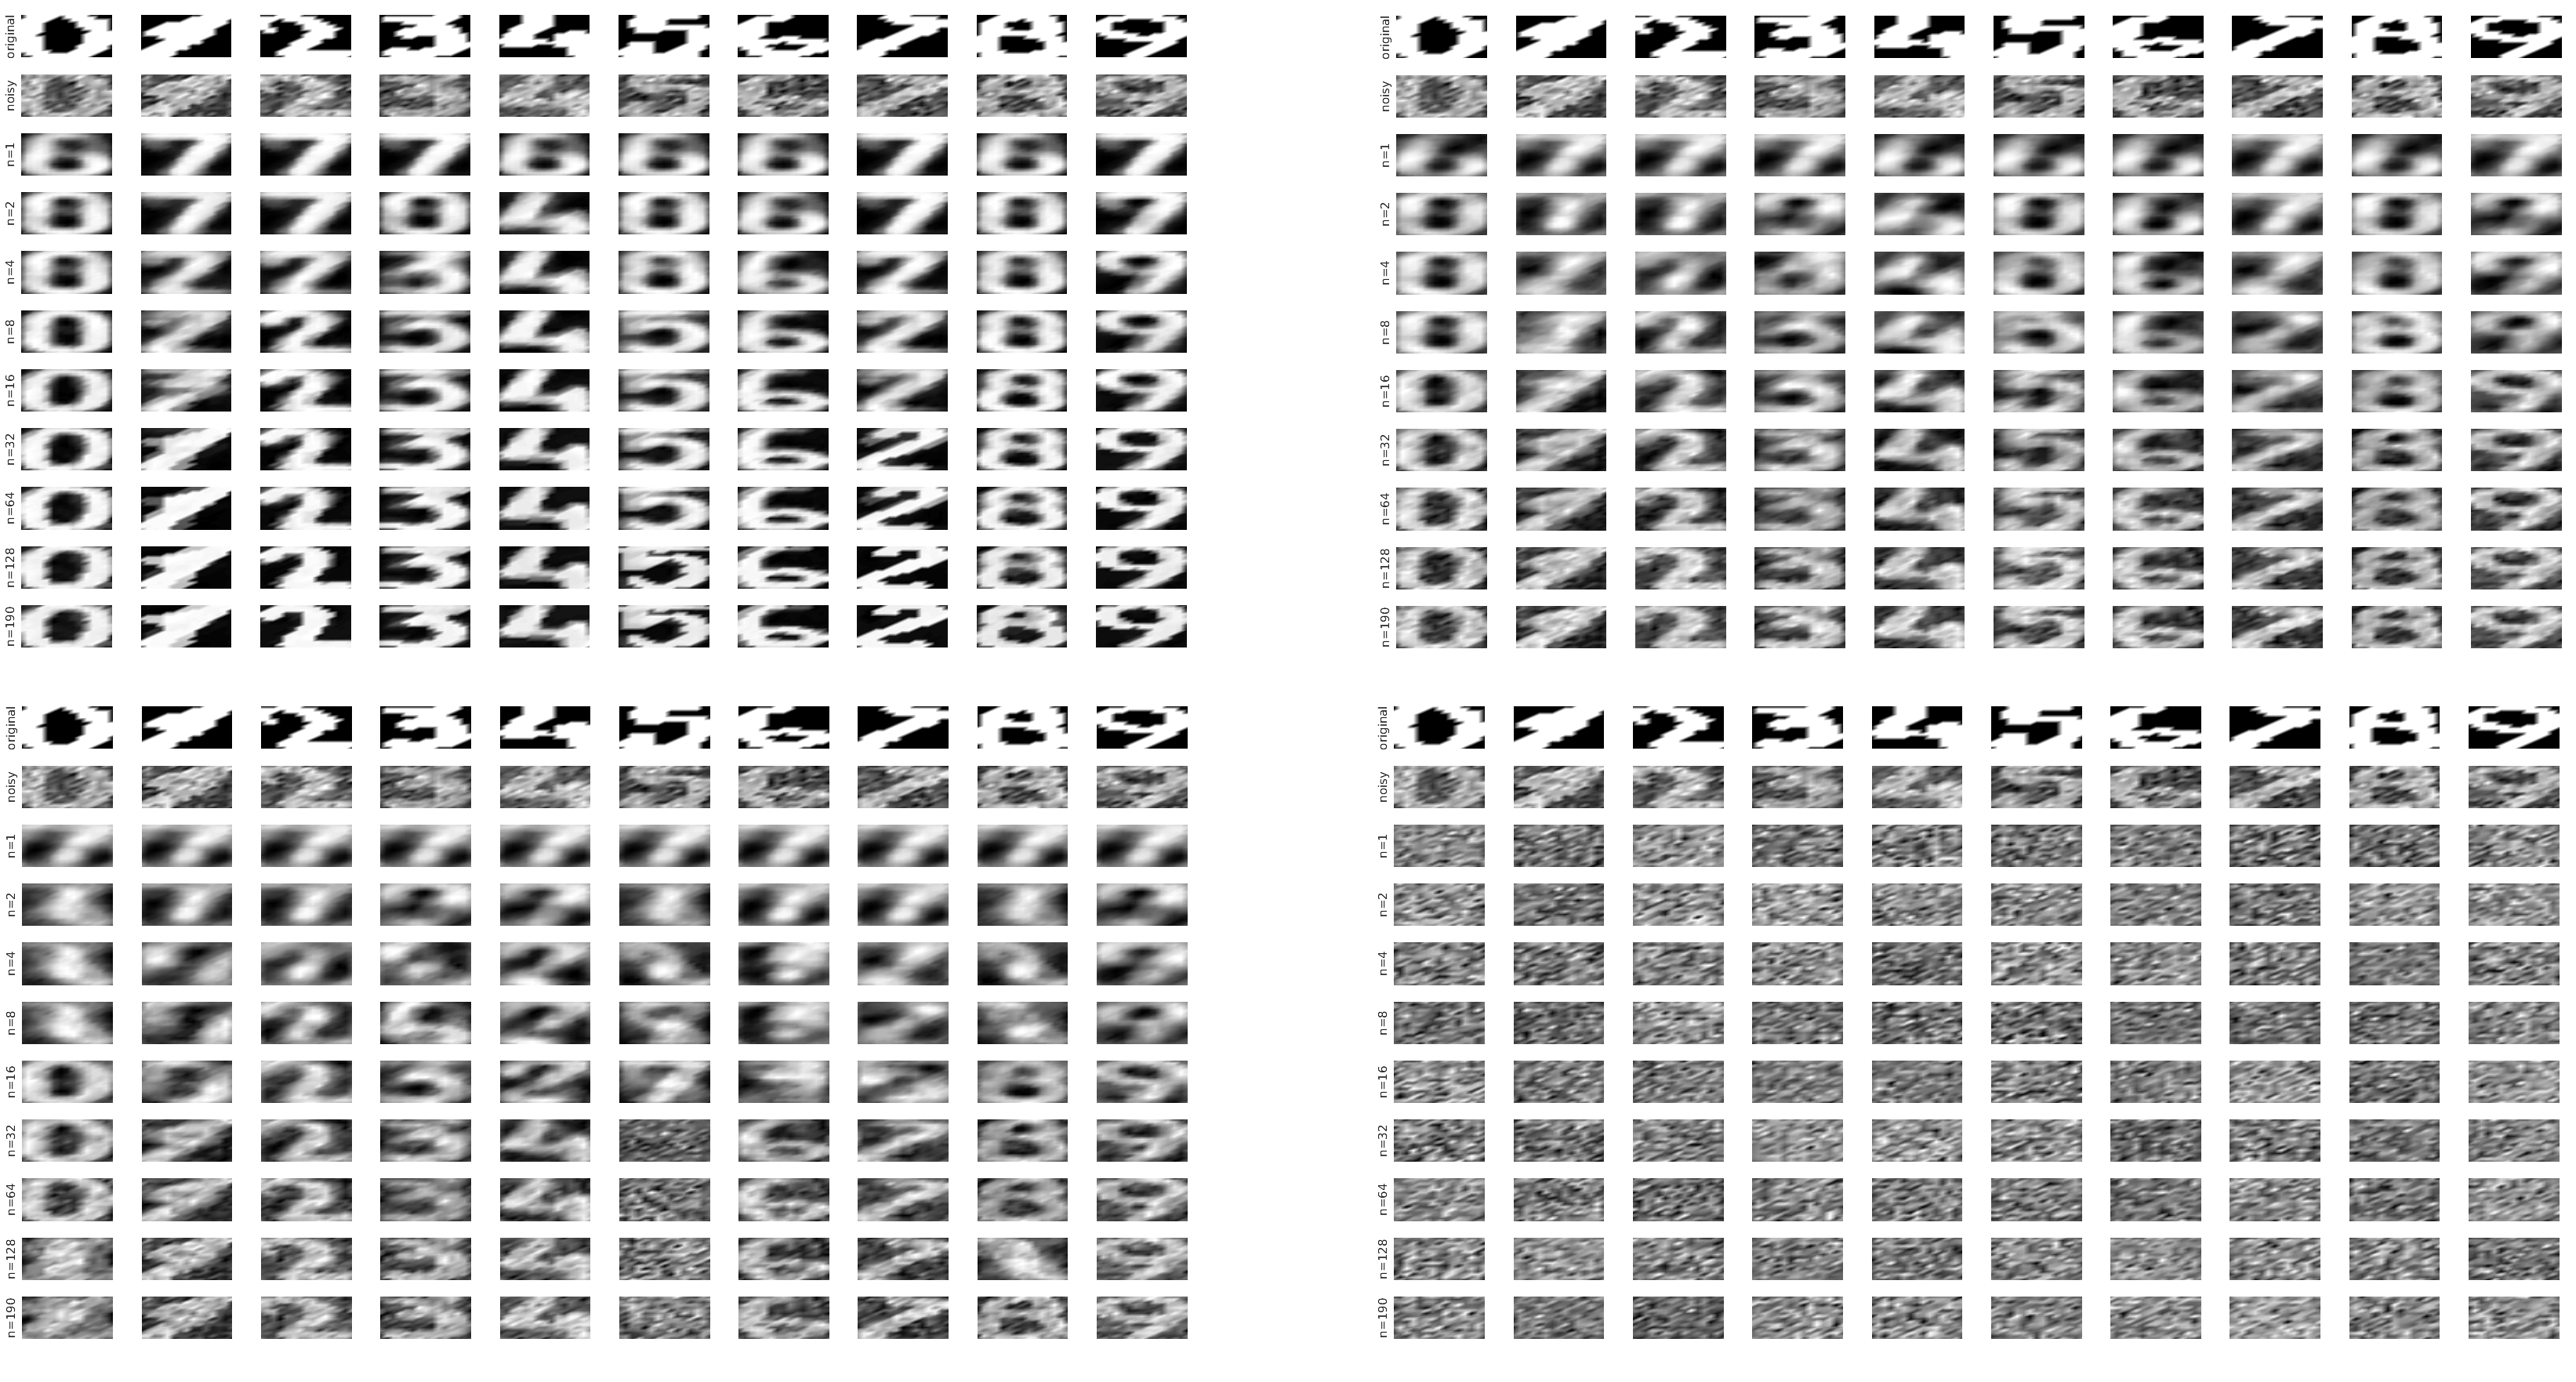
\includegraphics[scale=.15]{nndigits_all.png}
  \caption{Reconstruction different sigma (top to bottom, left to
    right: [50, 500, 5000, 50000]}
  \label{fig:nndigits_all}
\end{figure}

An example of linear vs. kernel PCA was given and commented in section
2, figure \ref{fig:digitsn_kernelpca} and \ref{fig:digitsn_linearpca}. 

\subsection{Shuttle (statlog)}

This exercise gives us a taste of what it is to work with large
dataset. As we know from the theory behind SVM, working with the dual
problem has great advantages, but requires to build the kernel matrix,
of size n-by-n. This matrix can be too large to store, or we may want
to work in the primal problem, which is of the dimension of the input
space. However, when we use a RBF kernel, we would need an explicit
construction of the feature map (infinite dimensional for the RBF
kernel). Working with fixed-size ls-svm allows us to get an
approximation of the feature map, and build our model using the primal
formulation.

For this exercise, one of the challenge was to deal with the sheer
amount of computations required for the fslssvm to complete. A first
attempt on my personal computer revealed a progress of less than 4\%
for 1 hour of computing time. I therefore used the VSC infrastructure,
where one node with 20 CPU cut down the computation time to around 3
hrs.

The results are displayed in figure \ref{fig:fslssvm_shuttle}. Note
that I divided the dataset between the training set and test set with
a ration of 70/30.

The errors are comparable for both approaches, and so was the time
estimate. The support vectors comparison however revealed that fewer
of them were necessary on average for the $SV\_L_0 norm$ than for the
FS-FLSSVM approach.

\begin{figure}[H]
  \centering
  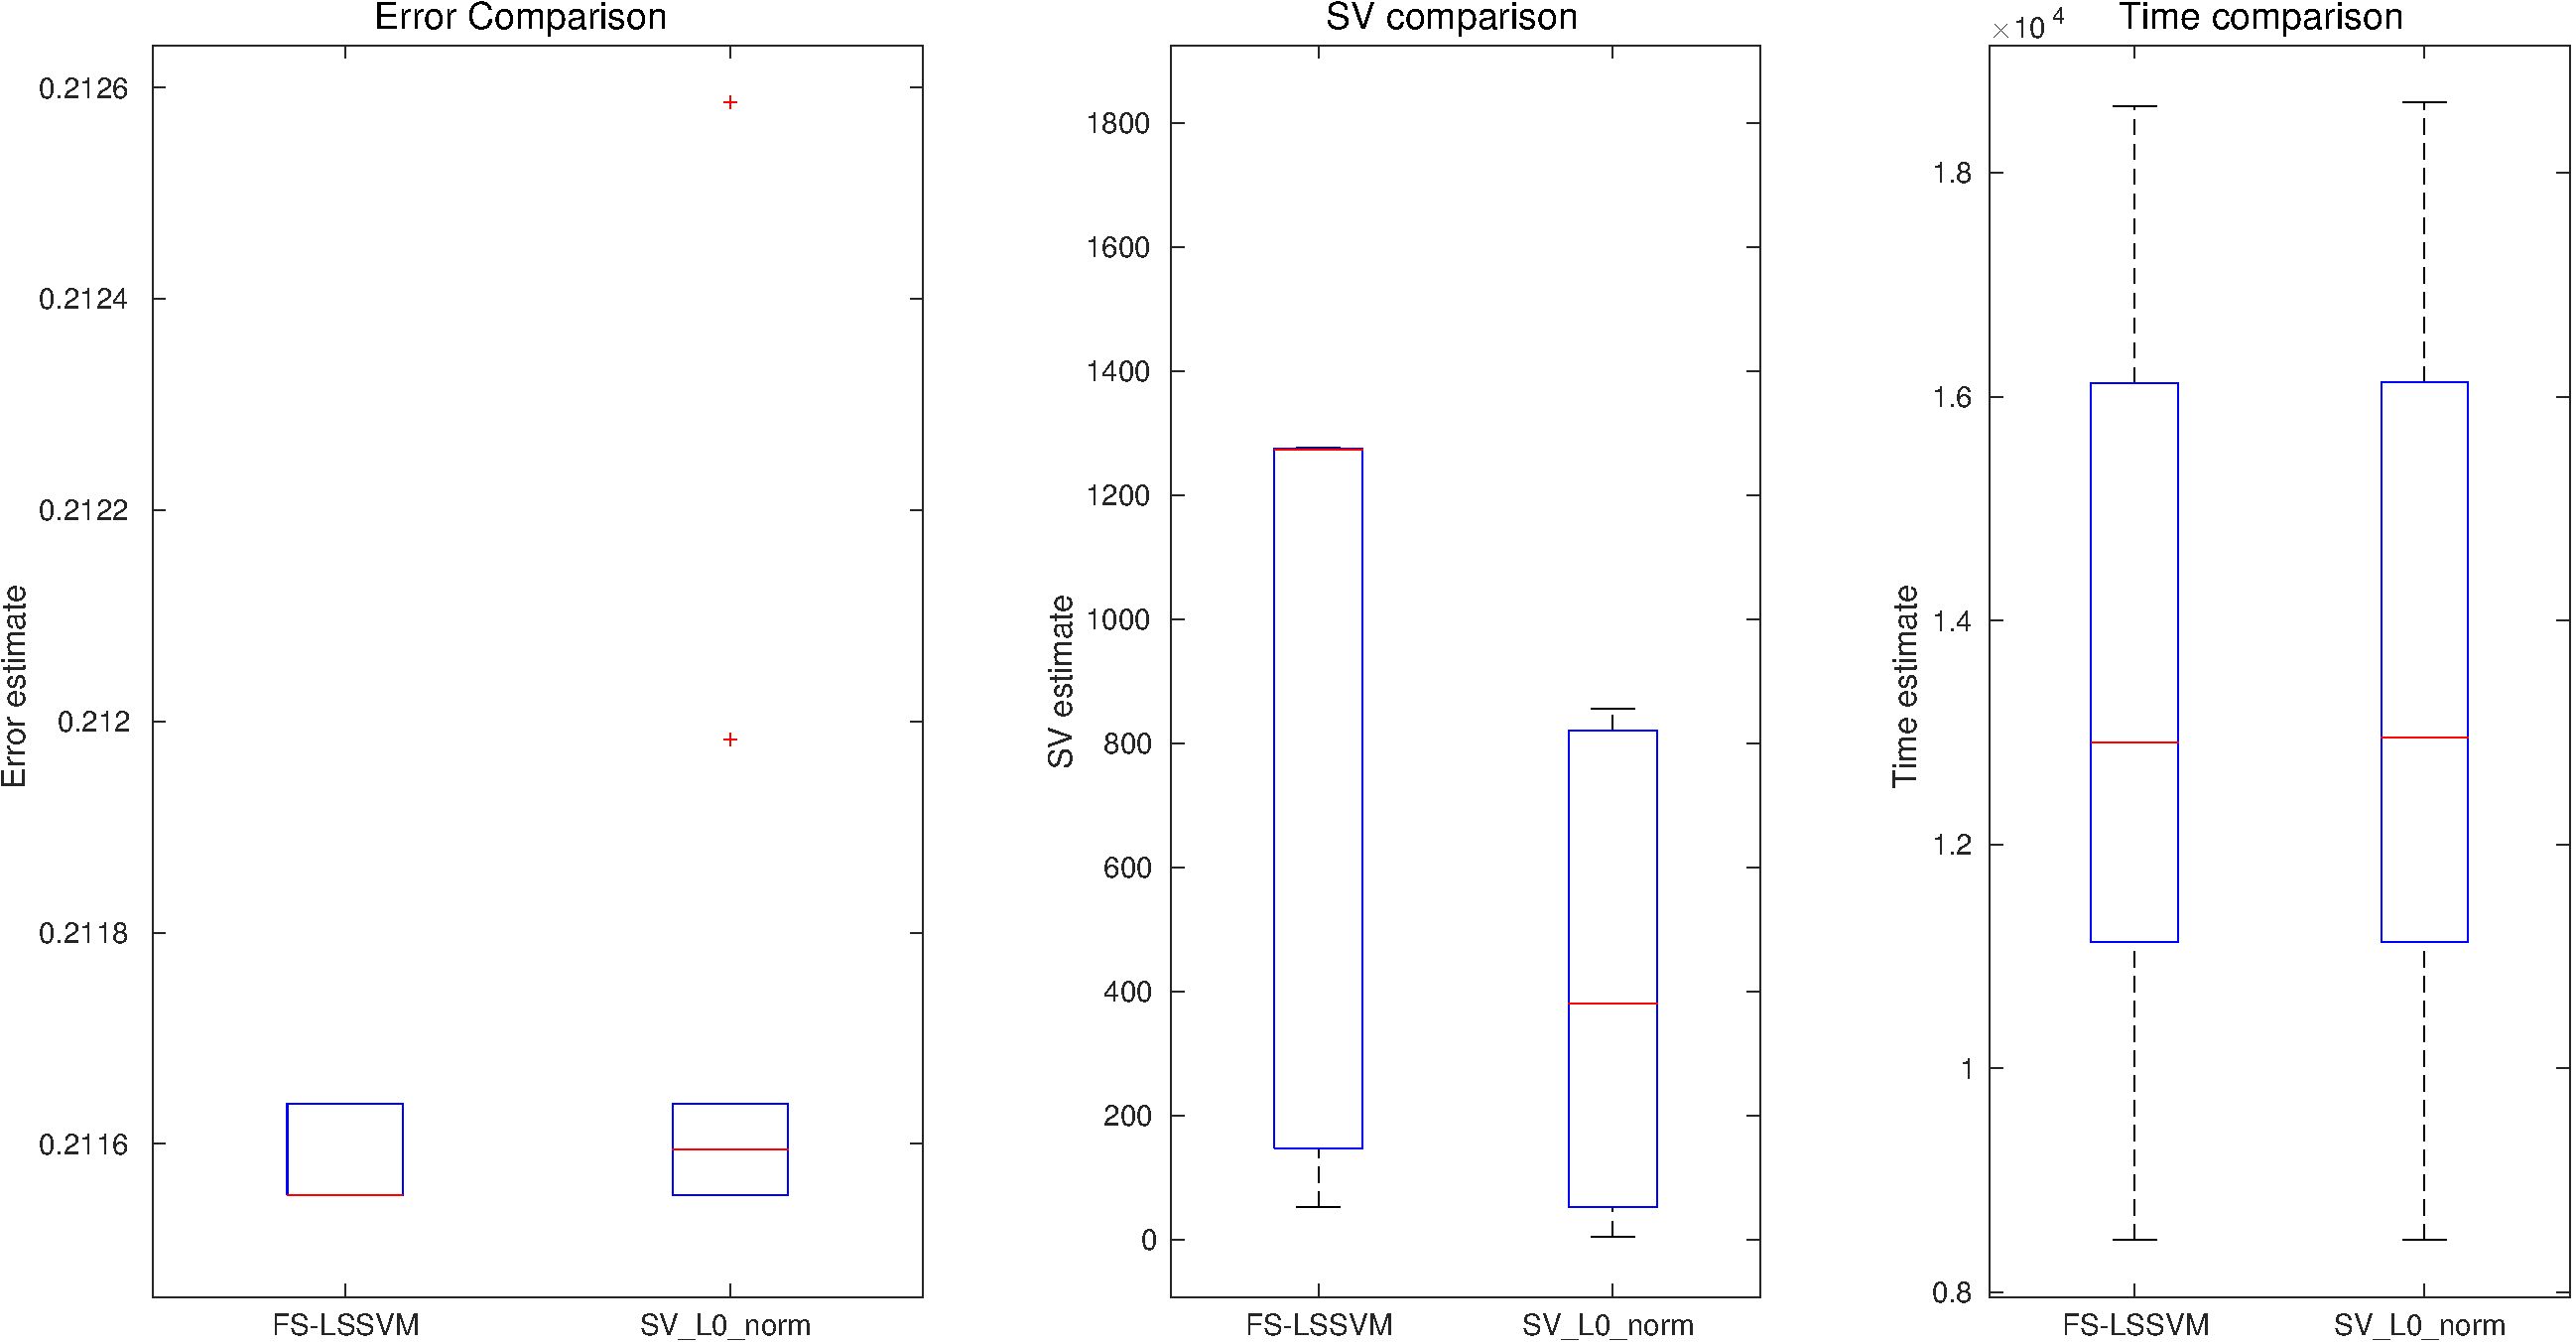
\includegraphics[scale=.40]{fslssvm_shuttle.pdf}
  \caption{Metrics comparison for fs-lssvm and l\_0}
  \label{fig:fslssvm_shuttle}
\end{figure}

\subsection{California}

The results are displayed in figure \ref{fig:fslssvm_california}. The
dataset was also divided in a 70\%/30\% scheme for the training and
test.

Similarly to the shuttle dataset, the time comparison does not reveal
major differences between the 2 approaches. The error is this time
noticeably different, with FS-LSSVM having an edge in terms of
accuracy. The number of SV is in accordance with the previous section,
where we also found a higher number of SV needed for the FS-LSSVM
approach.

\begin{figure}[H]
  \centering
  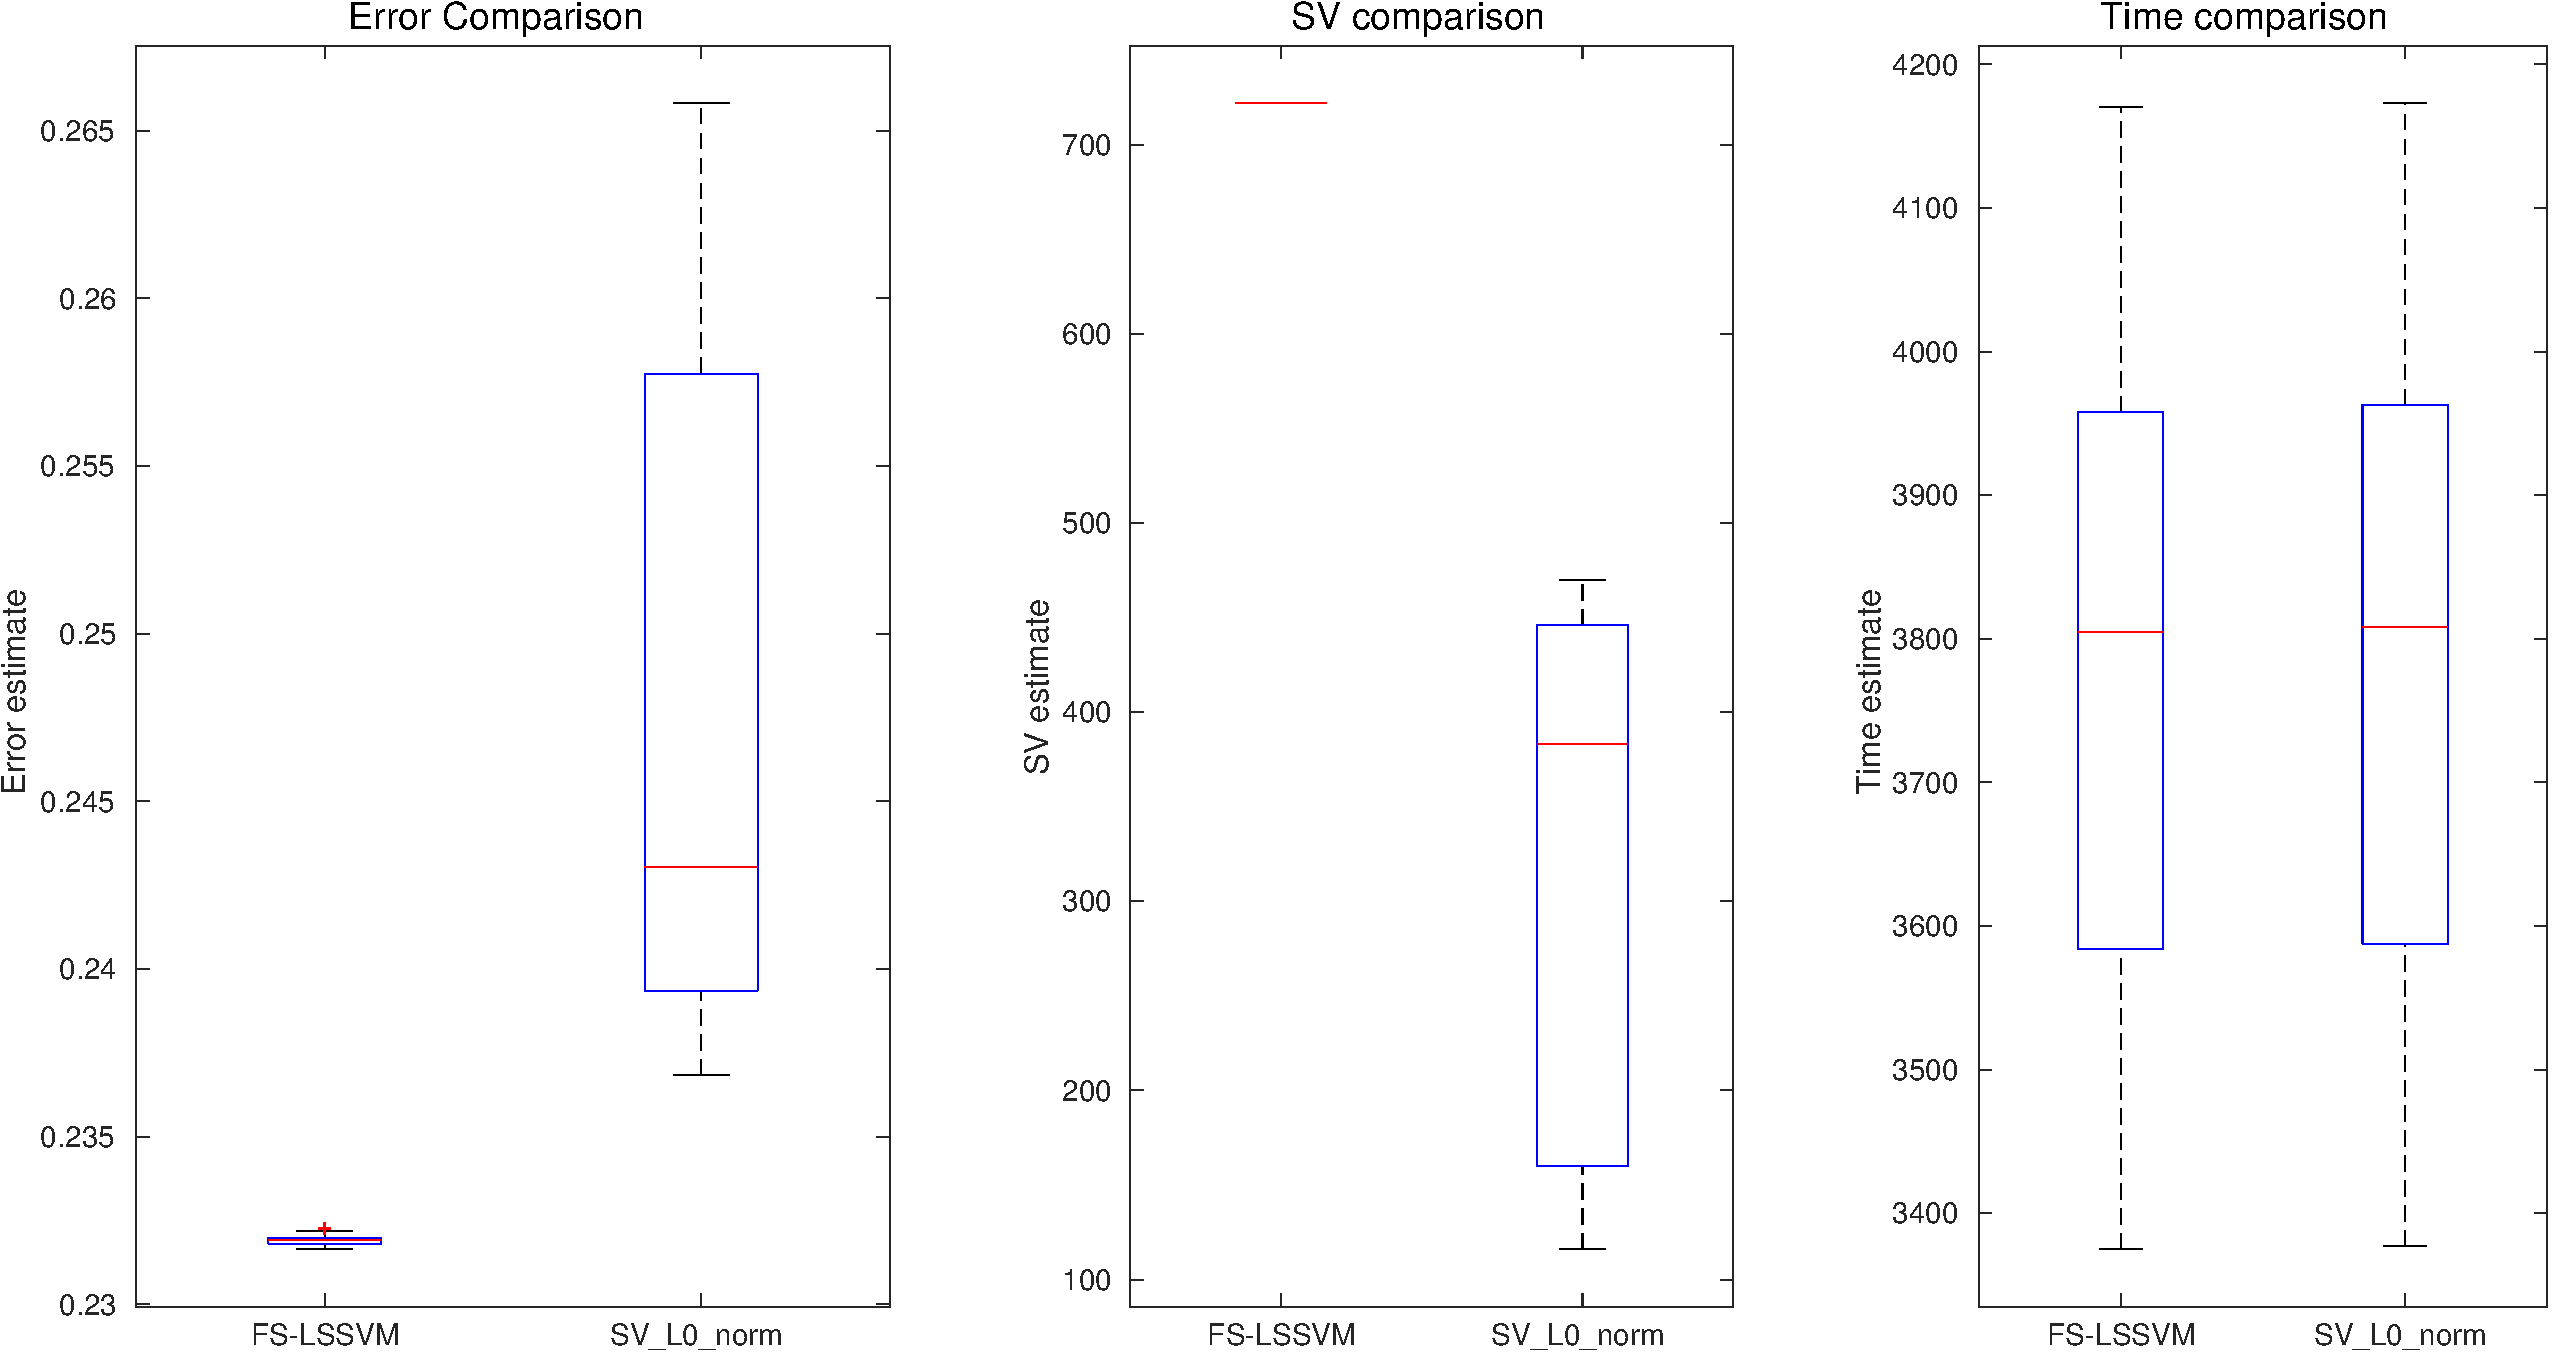
\includegraphics[scale=.40]{fslssvm_california.pdf}
  \caption{Metrics comparison for fs-lssvm and l\_0}
  \label{fig:fslssvm_california}
\end{figure}
%\bibliographystyle{ieeetr} \bibliography{bib-db}
\end{document}
